\section{Histograms~\label{sec:sodb9_hist}} 
This section exhibits histograms on the EMPv5 data obtained when 
the task length of INC increases from 1 second to 2048 seconds. 
The detailed description of the base data is from Table~\ref{tab:exp_notes}.

\subsection{ET}

\begin{figure}[hp!]
	\centering
	\subfigure[ET frequency on INC1]{
		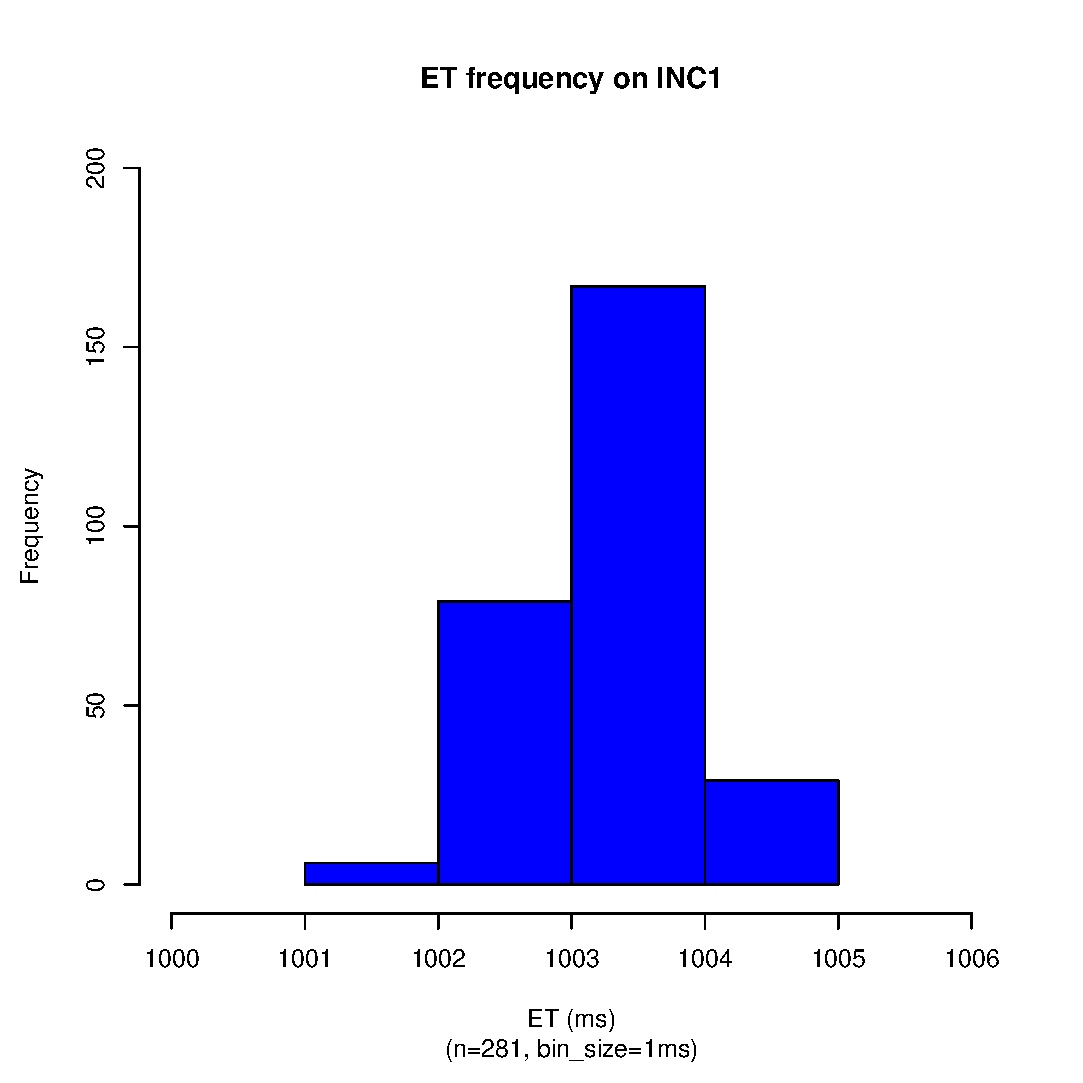
\includegraphics[scale=0.43]{sodb9/1_sec_et_hist_v5.eps}
		\label{fig:inc1_et_hist_v5}
	}
	\subfigure[ET frequency on INC2]{
		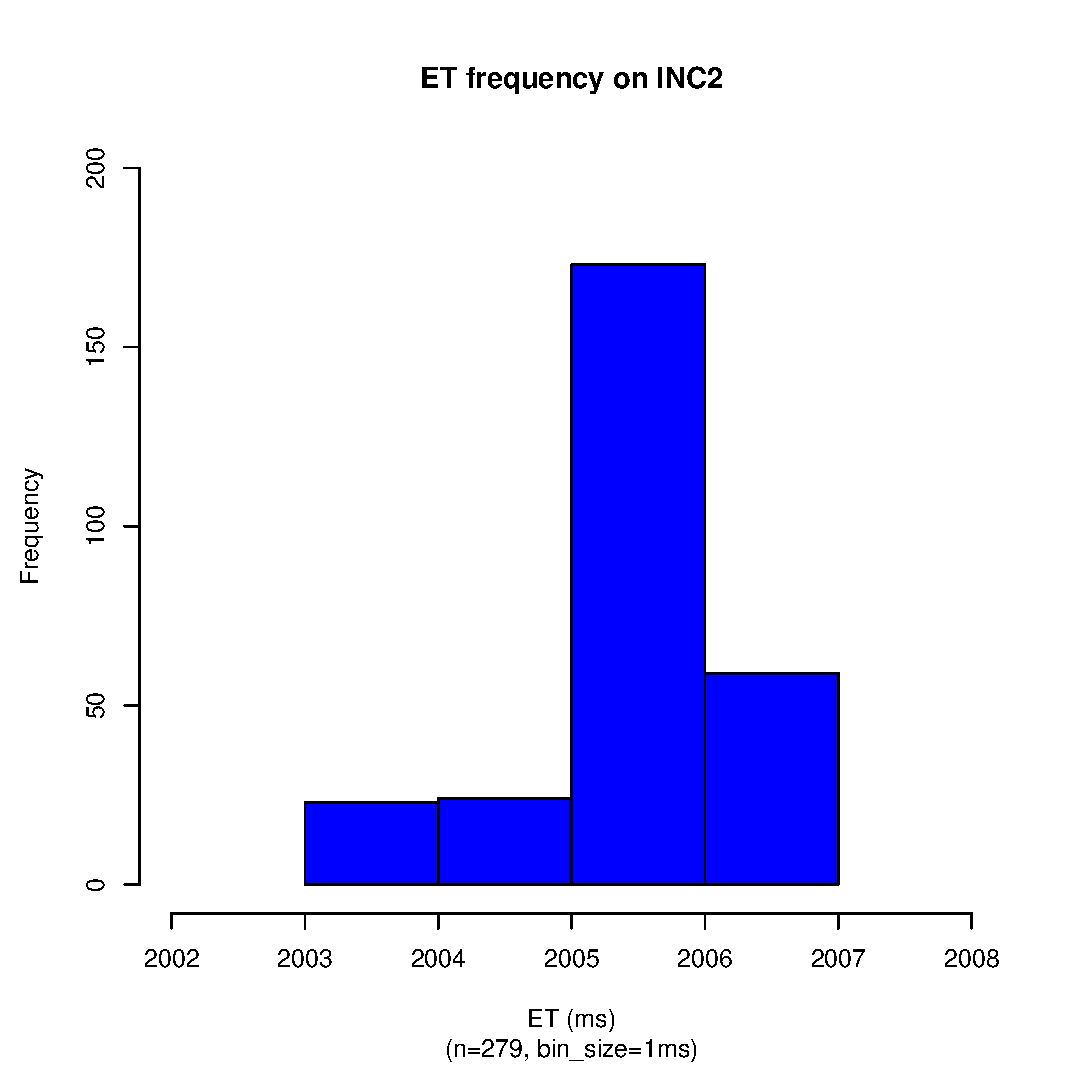
\includegraphics[scale=0.43]{sodb9/2_sec_et_hist_v5.eps}
		\label{fig:inc2_et_hist_v5}
	}
	\subfigure[ET frequency on INC4]{
		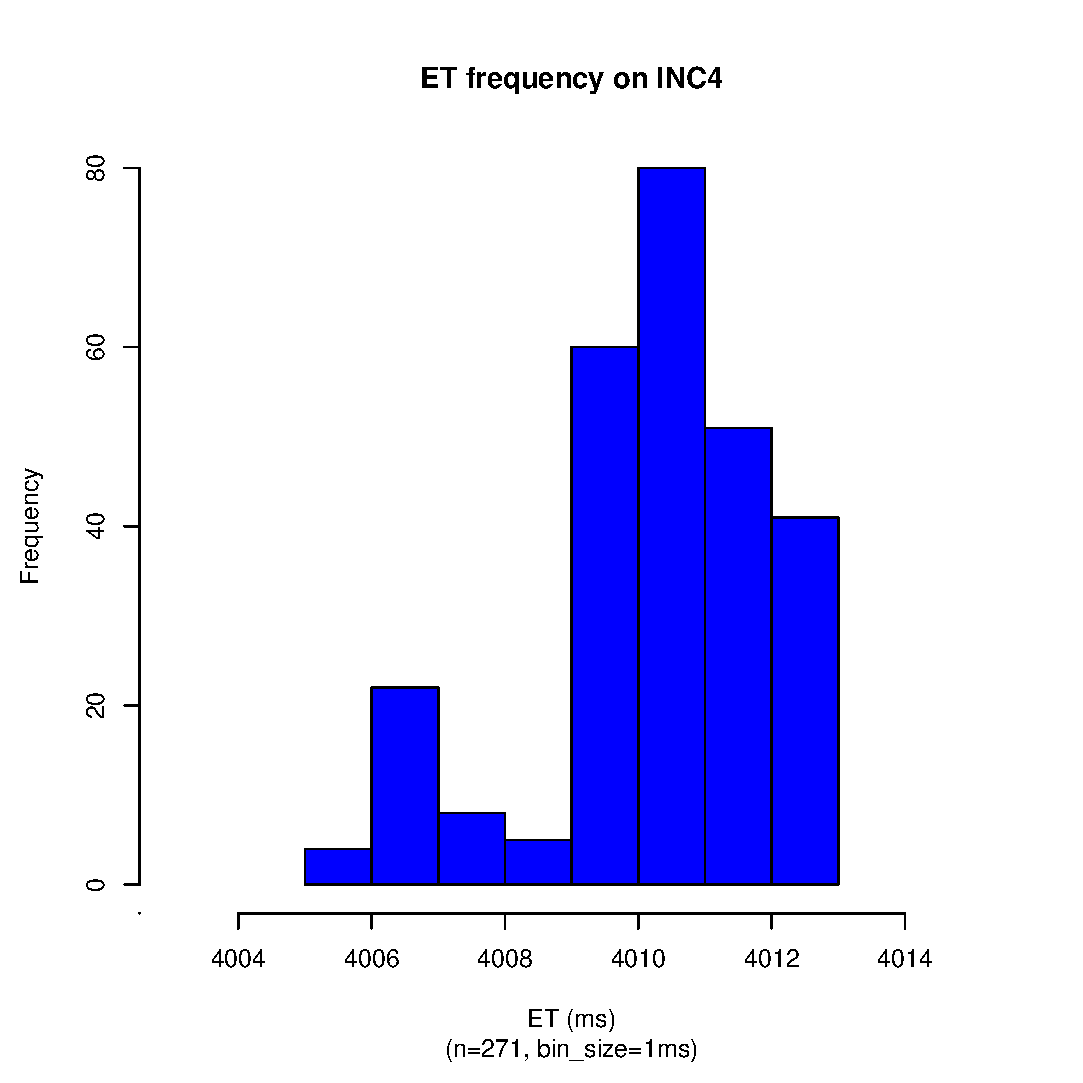
\includegraphics[scale=0.43]{sodb9/4_sec_et_hist_v5.eps}
		\label{fig:inc4_et_hist_v5}
	}
	\subfigure[ET frequency on INC8]{
		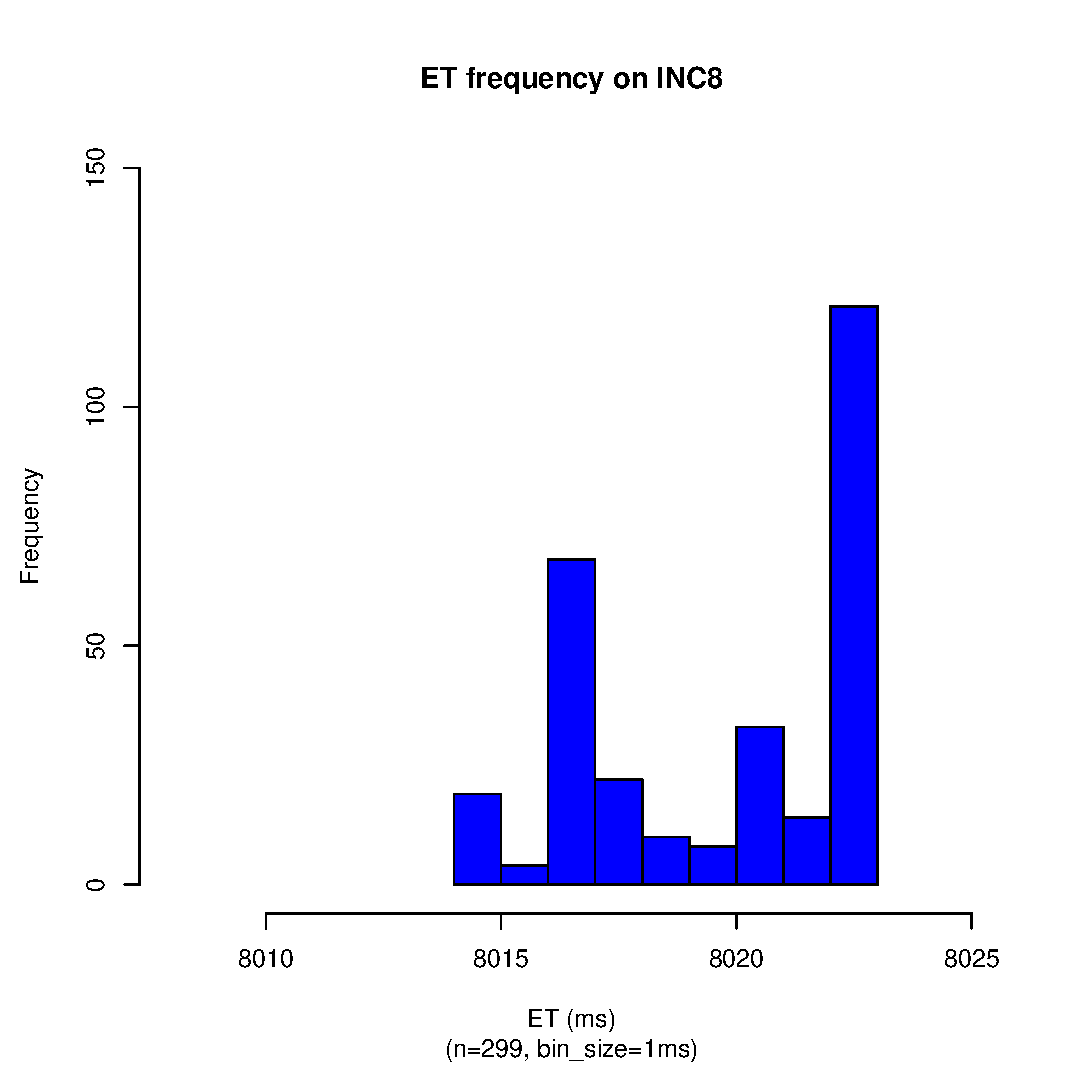
\includegraphics[scale=0.43]{sodb9/8_sec_et_hist_v5.eps}
		\label{fig:inc8_et_hist_v5}
	}
	\caption{ET Histograms of INC1 ... INC8~\label{fig:s9_et_hist1}}
\end{figure}

\begin{figure}[hp!]
	\centering
	\subfigure[ET frequency on INC16]{
		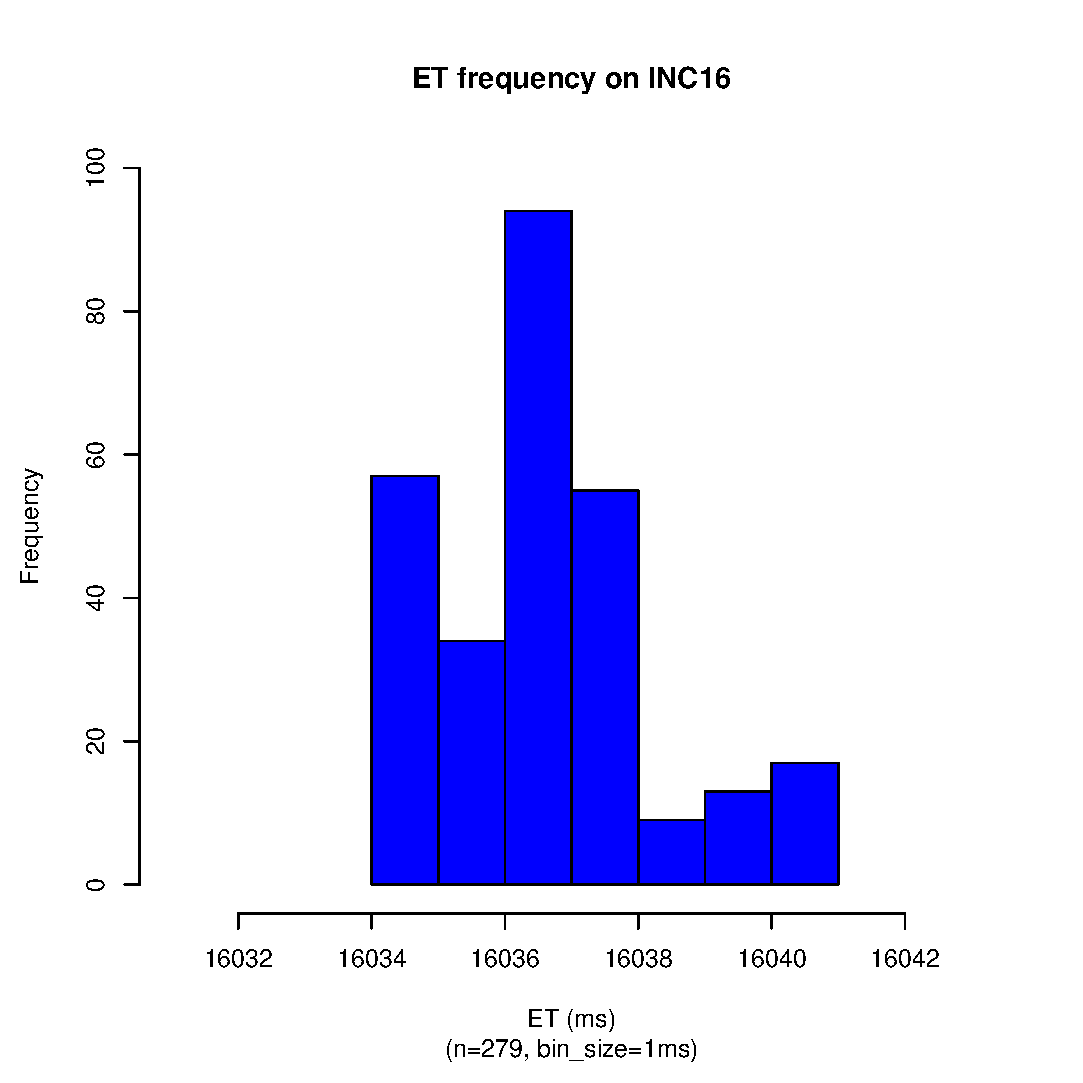
\includegraphics[scale=0.43]{sodb9/16_sec_et_hist_v5.eps}
		\label{fig:inc16_et_hist_v5}
	}
	\subfigure[ET frequency on INC32]{
		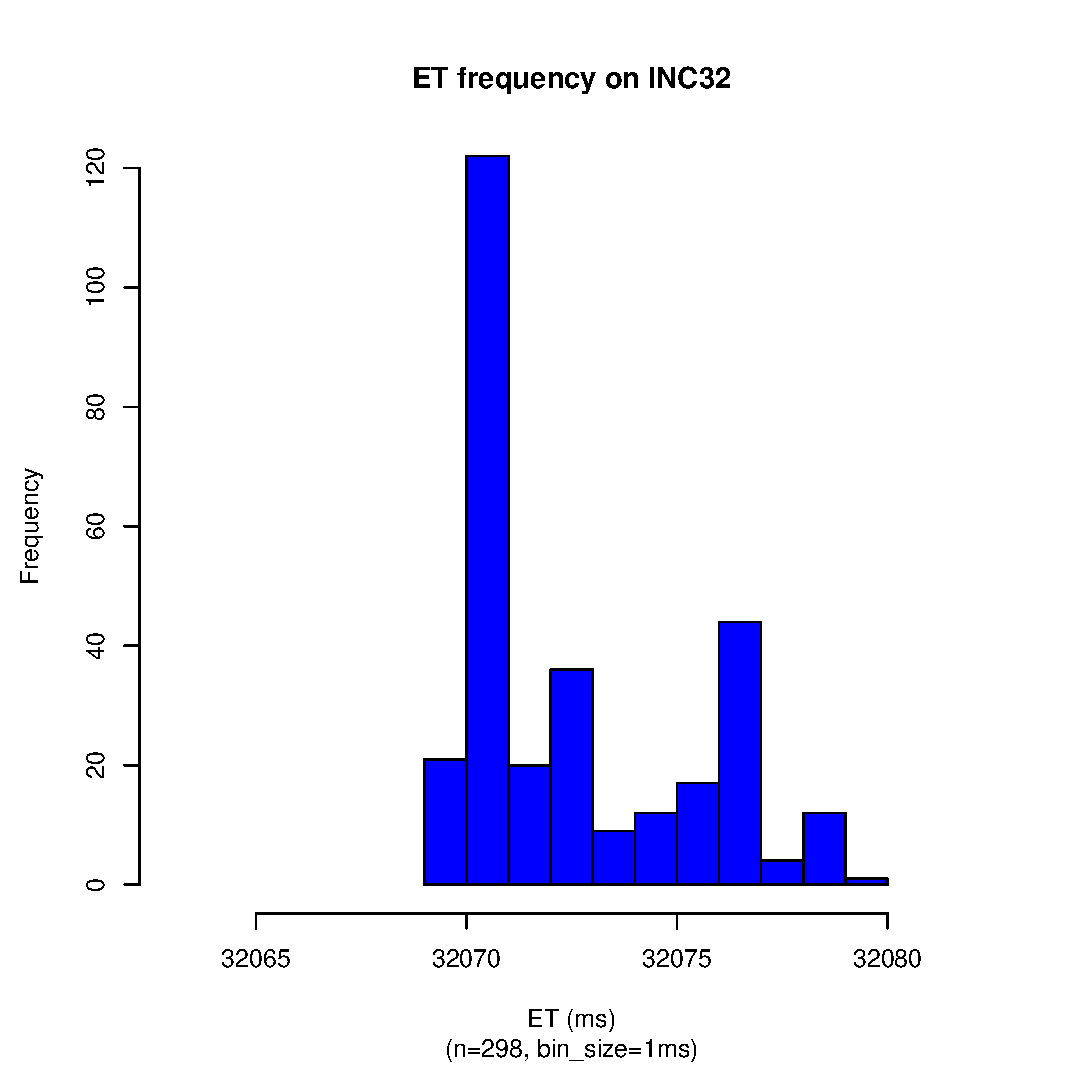
\includegraphics[scale=0.43]{sodb9/32_sec_et_hist_v5.eps}
		\label{fig:inc32_et_hist_v5}
	}
	\subfigure[ET frequency on INC64]{
		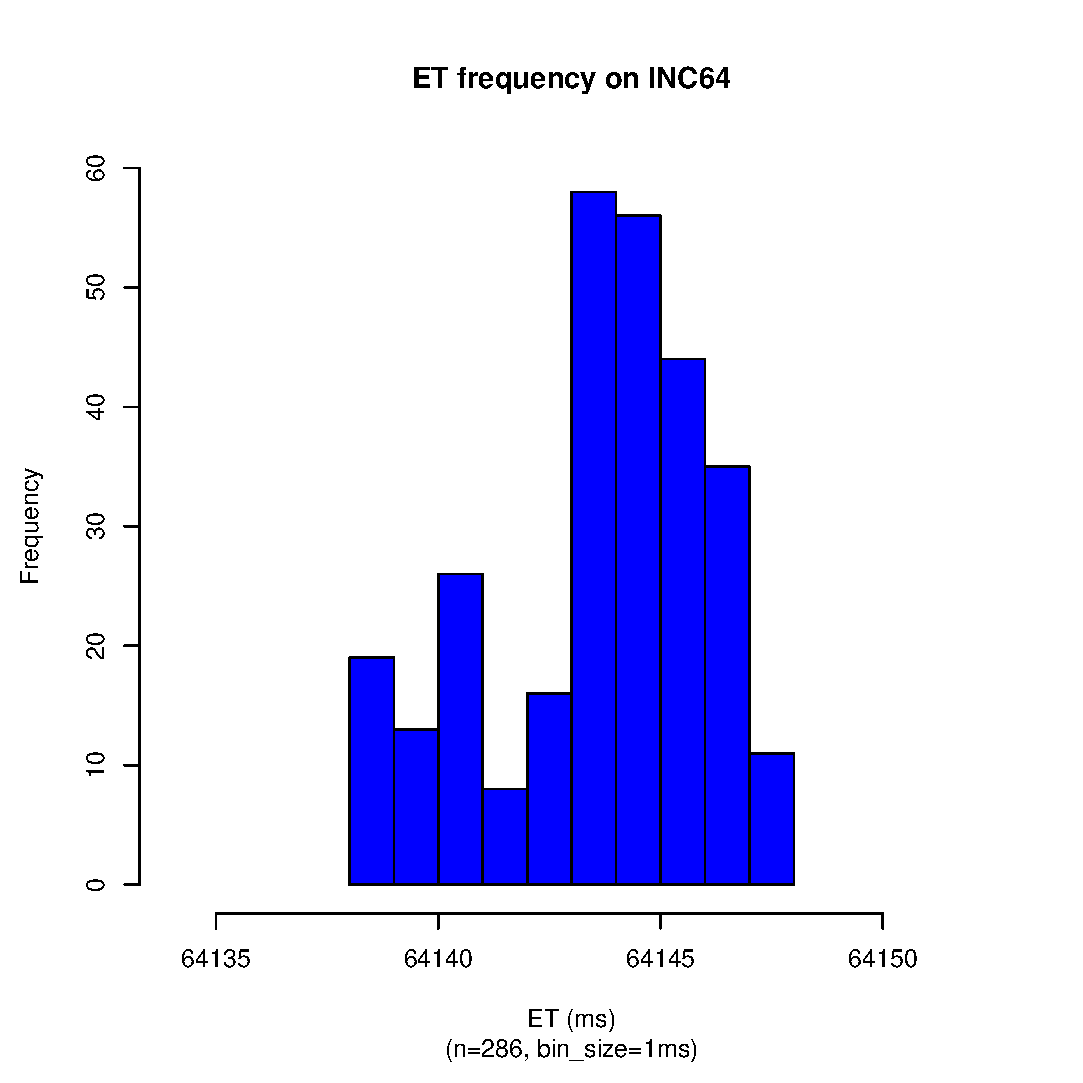
\includegraphics[scale=0.43]{sodb9/64_sec_et_hist_v5.eps}
		\label{fig:inc64_et_hist_v5}
	}
	\caption{ET Histograms of INC16 ... INC64~\label{fig:s9_et_hist2}}
\end{figure}

\begin{figure}[hp!]
	\centering
	\subfigure[ET frequency on INC128]{
		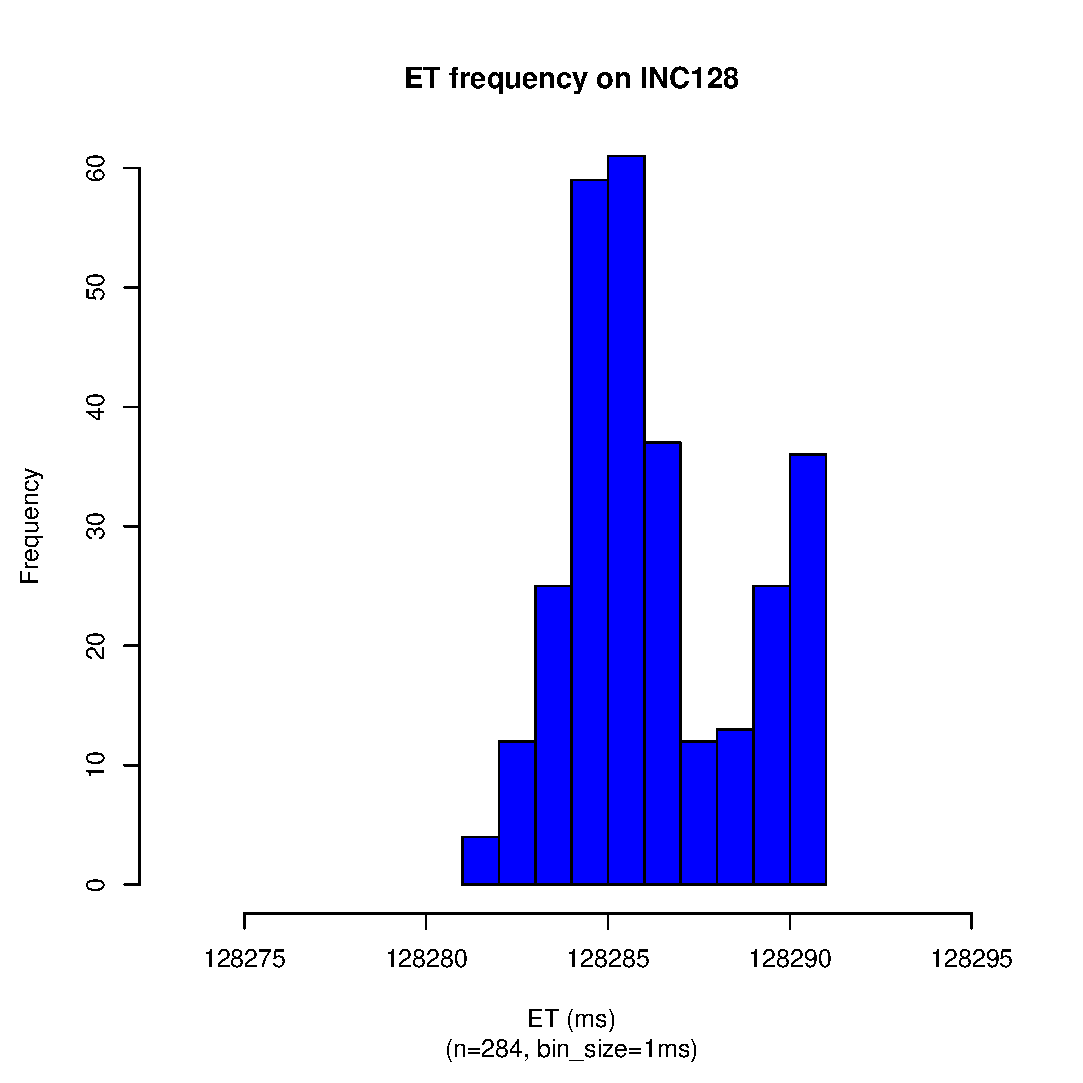
\includegraphics[scale=0.43]{sodb9/128_sec_et_hist_v5.eps}
		\label{fig:inc128_et_hist_v5}
	}
	\subfigure[ET frequency on INC256]{
		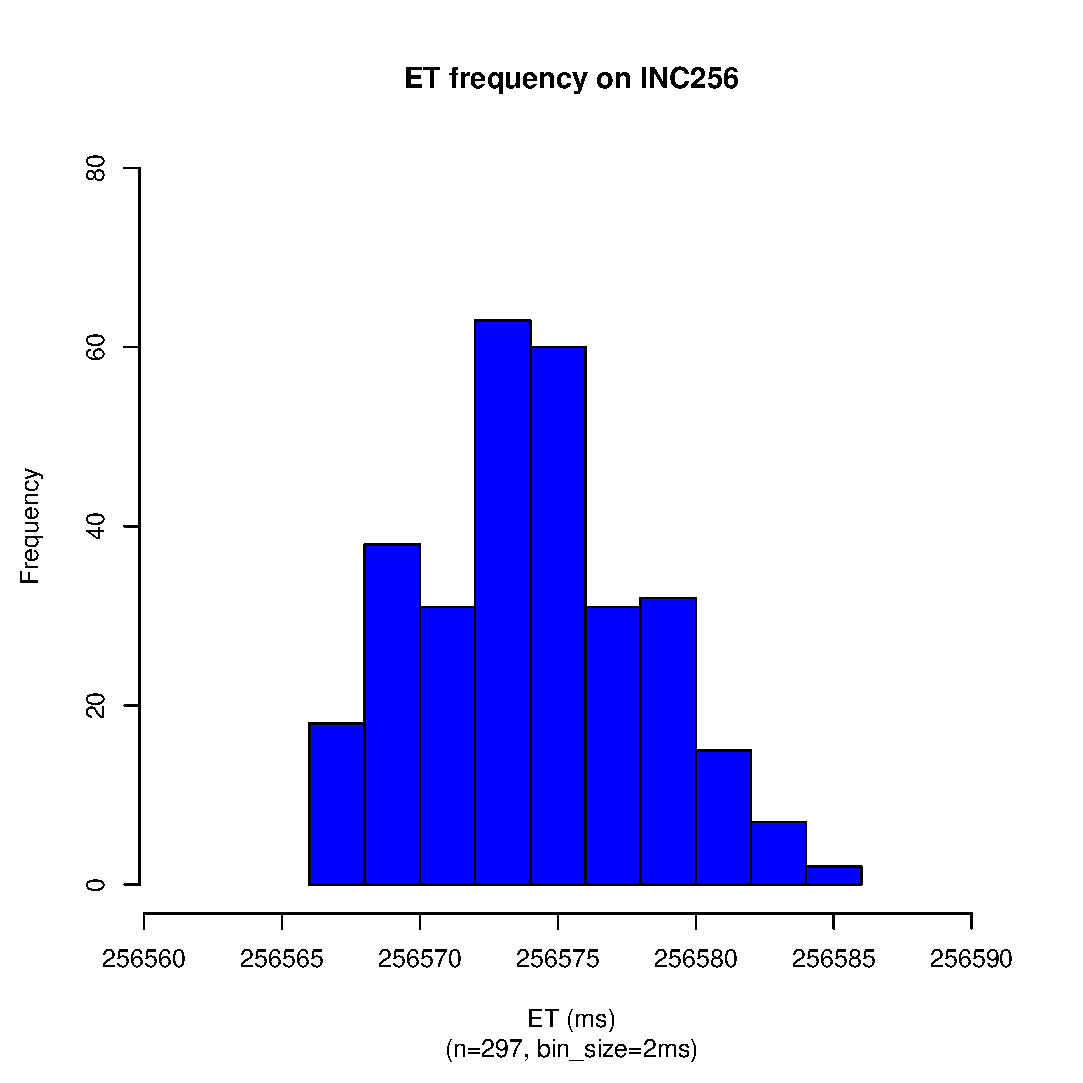
\includegraphics[scale=0.43]{sodb9/256_sec_et_hist_v5.eps}
		\label{fig:inc256_et_hist_v5}
	}
	\subfigure[ET frequency on INC512]{
		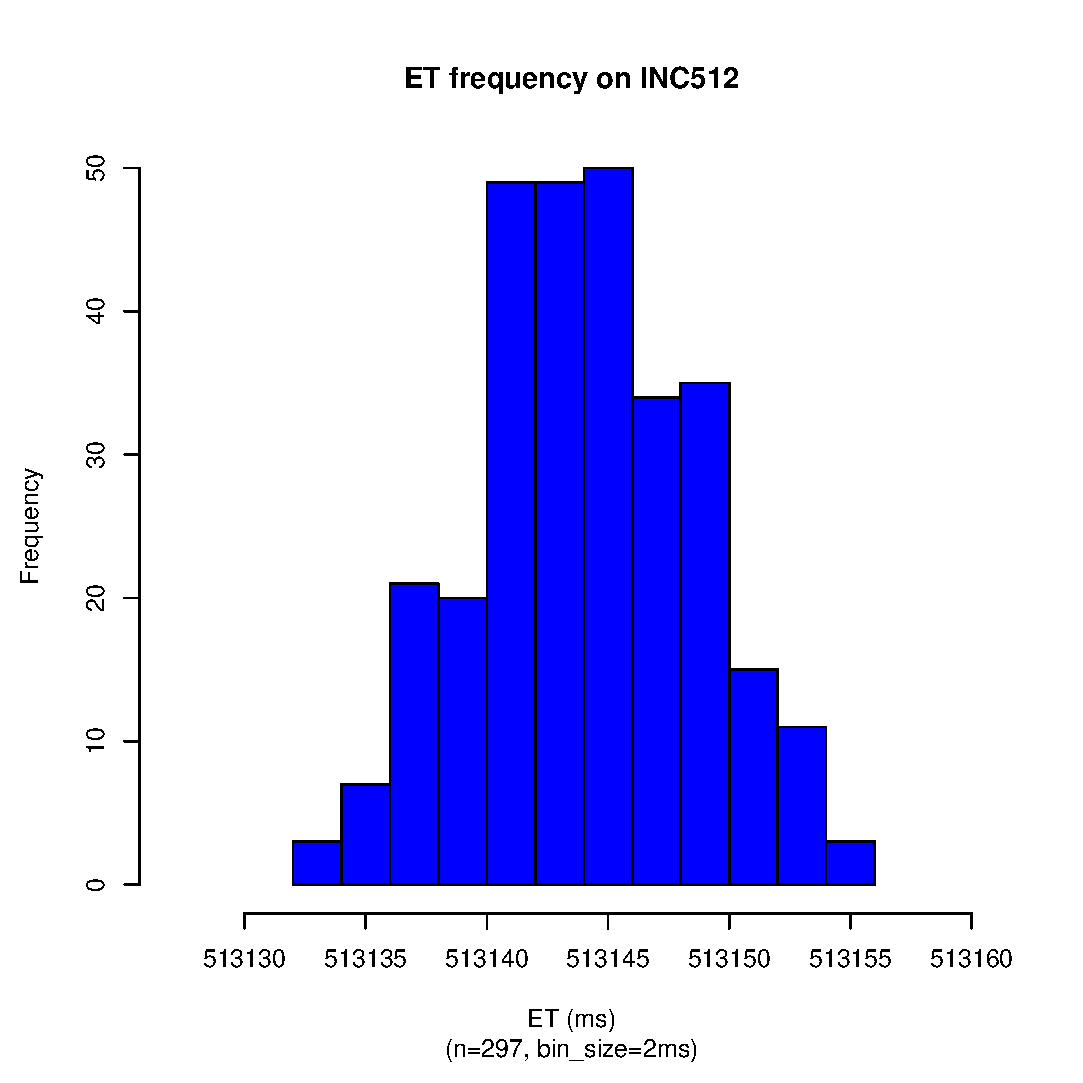
\includegraphics[scale=0.43]{sodb9/512_sec_et_hist_v5.eps}
		\label{fig:inc512_et_hist_v5}
	}
	\subfigure[ET frequency on INC1024]{
		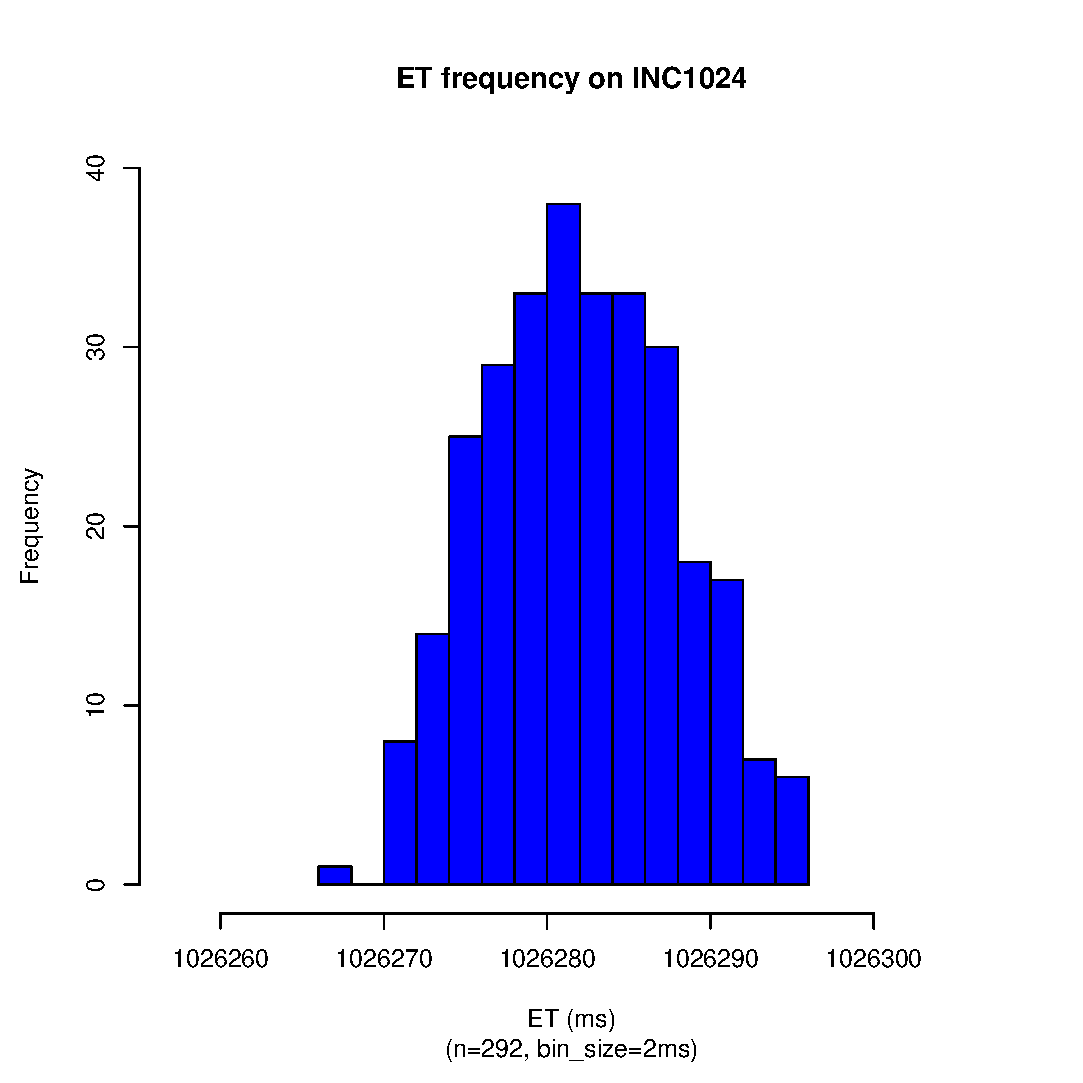
\includegraphics[scale=0.43]{sodb9/1024_sec_et_hist_v5.eps}
		\label{fig:inc1024_et_hist_v5}
	}
	\caption{ET Histograms of INC128 ... INC1024~\label{fig:s9_et_hist3}}
\end{figure}

\pagebreak

\begin{figure}[hp!]
	\centering
	\subfigure[ET frequency on INC2048]{
		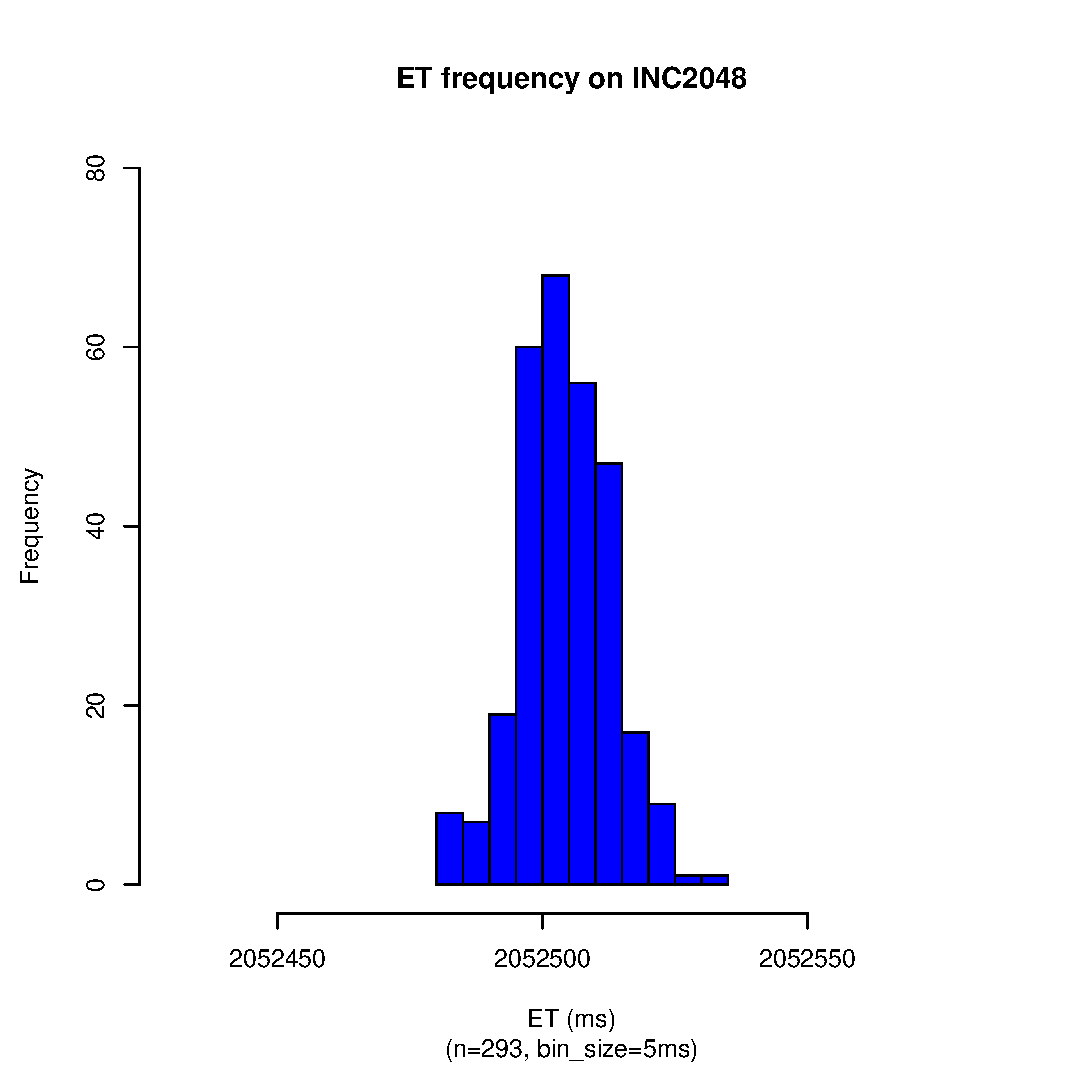
\includegraphics[scale=0.43]{sodb10/2048_sec_et_hist_v5.eps}
		\label{fig:inc2048_et_hist_v5}
	}
	\subfigure[ET frequency on INC4096]{
		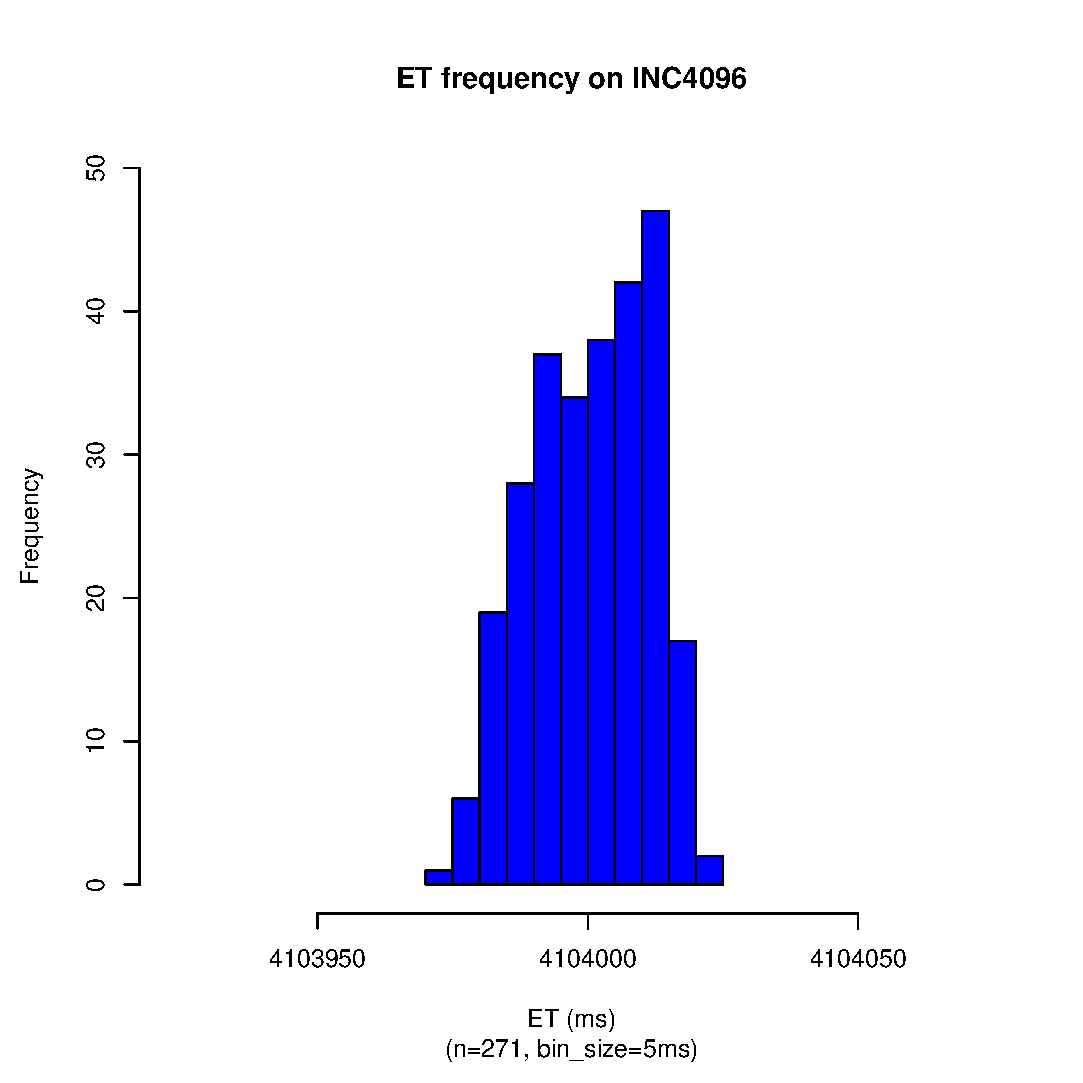
\includegraphics[scale=0.43]{sodb12/4096_sec_et_hist_v5.eps}
		\label{fig:inc4096_et_hist_v5}
	}
	\subfigure[ET frequency on INC8192]{
		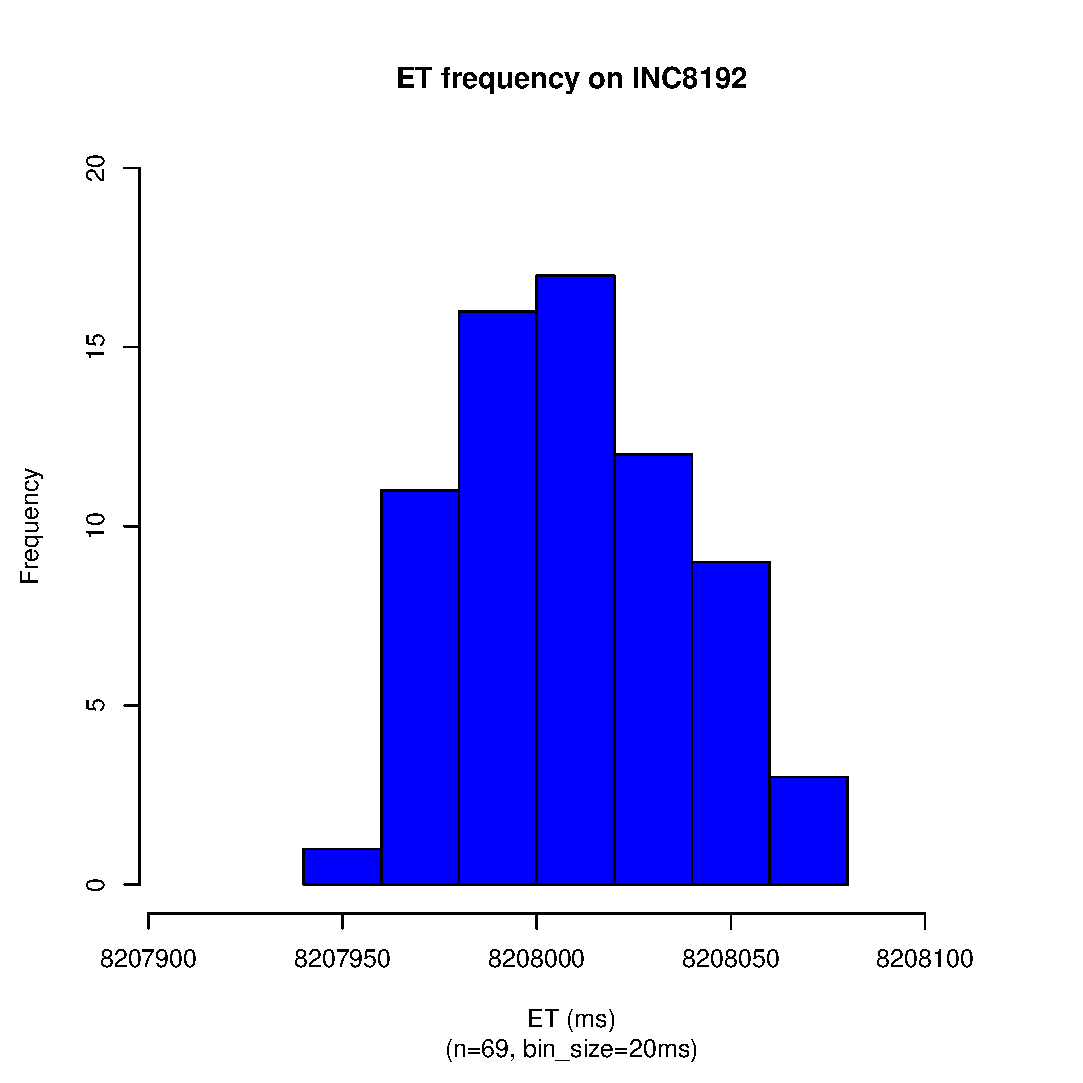
\includegraphics[scale=0.43]{sodb12/8192_sec_et_hist2_v5.eps}
		\label{fig:inc8192_et_hist_v5}
	}
	\subfigure[ET frequency on INC16384]{
		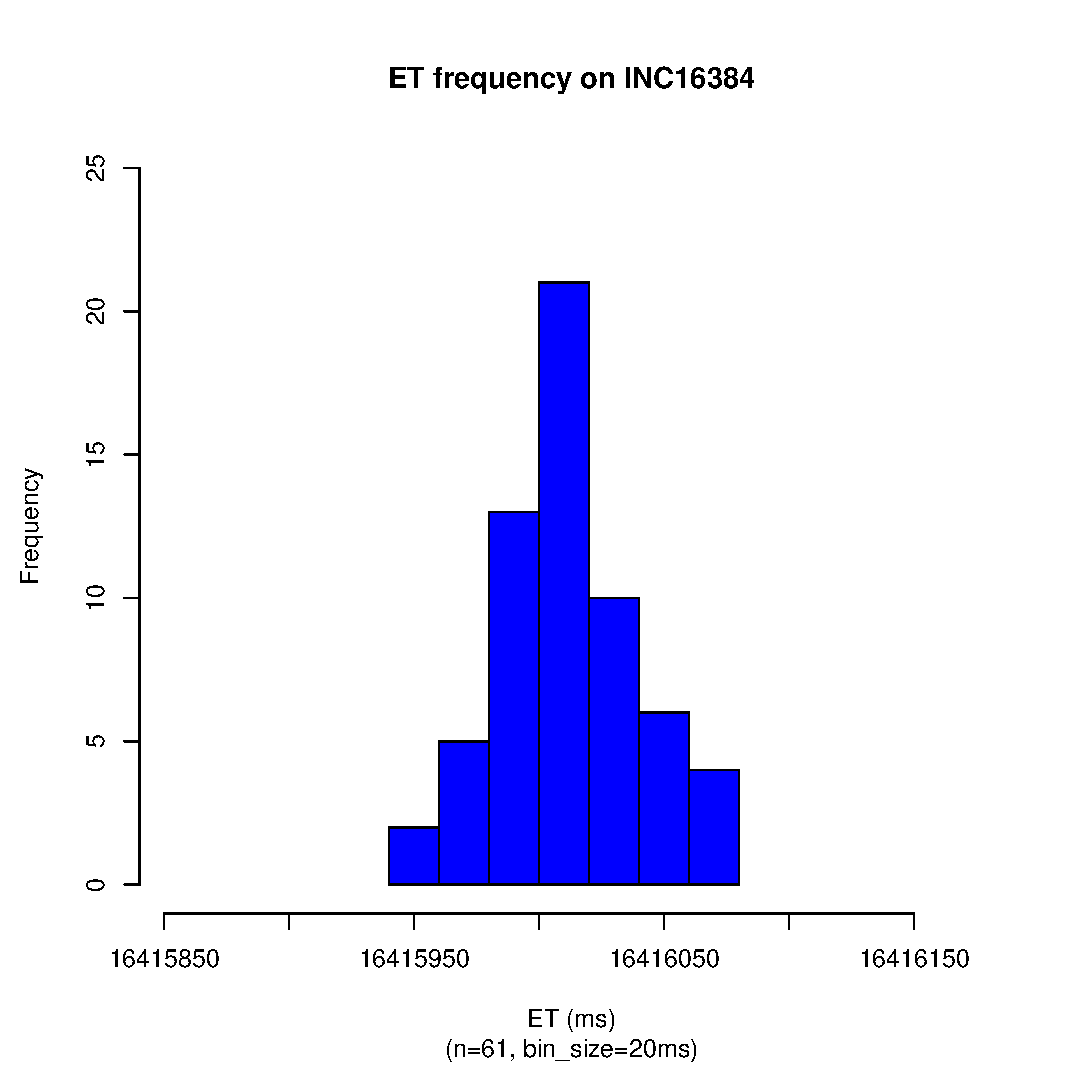
\includegraphics[scale=0.43]{sodb12/16384_sec_et_hist2_v5.eps}
		\label{fig:inc16384_et_hist_v5}
	}
	\caption{ET Histograms of INC2048 ... INC16384~\label{fig:s9_et_hist4}}
\end{figure}

%\pagebreak
%
%\begin{figure}[hp!]
%	\centering
%	\subfigure[ET frequency on INC8192]{
%		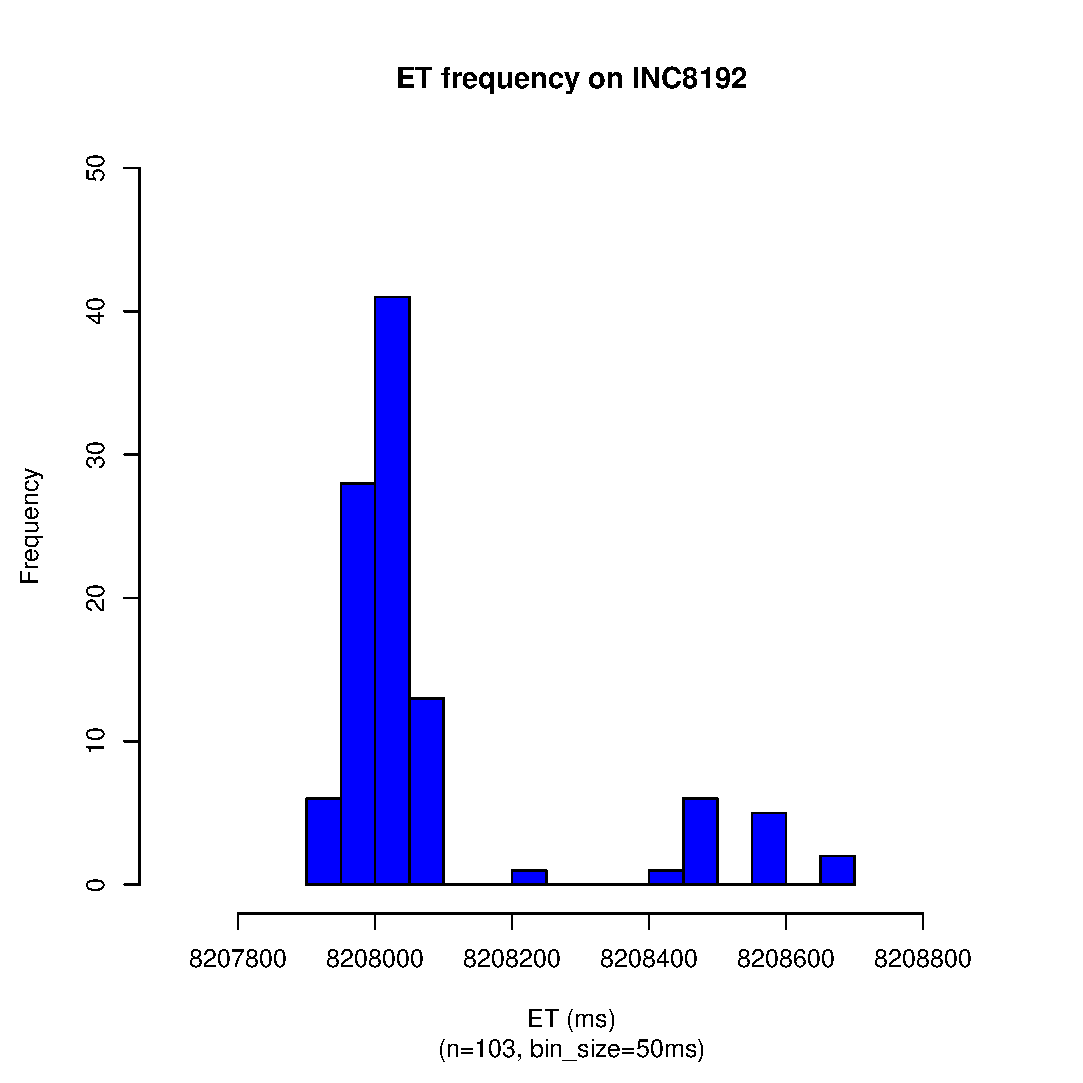
\includegraphics[scale=0.43]{sodb12/8192_sec_et_hist_v5.eps}
%		\label{fig:inc8192_et_hist_all_v5}
%	}
%	\subfigure[ET frequency on INC16384]{
%		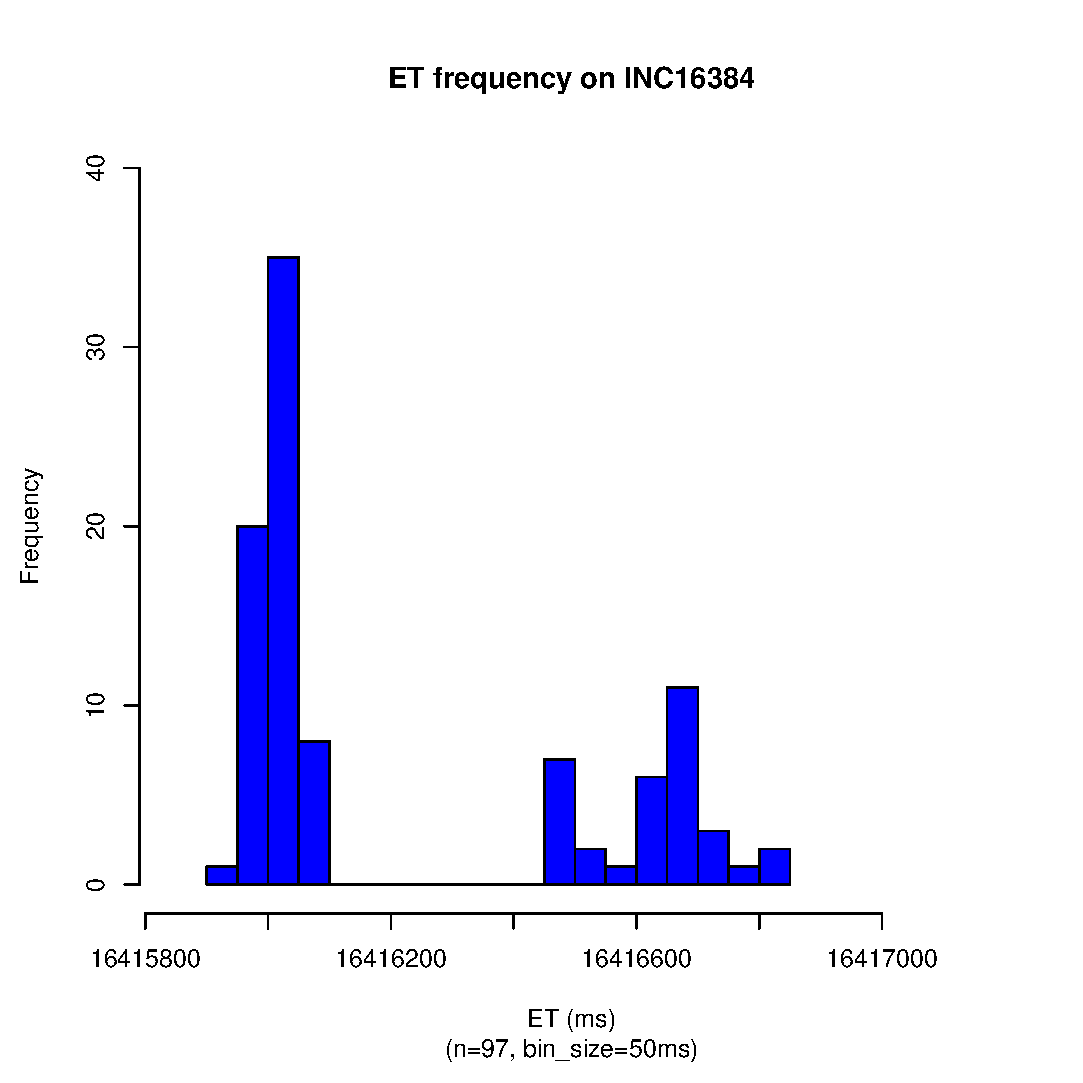
\includegraphics[scale=0.43]{sodb12/16384_sec_et_hist_v5.eps}
%		\label{fig:inc16384_et_hist_all_v5}
%	}
%	\caption{ET Histograms of INC8192... INC16384 [combined with 2015's run]~\label{fig:s9_et_hist5}}
%\end{figure}

\newpage

\subsection{PT}

\begin{figure}[hp!]
	\centering
	\subfigure[PT frequency on INC1]{
		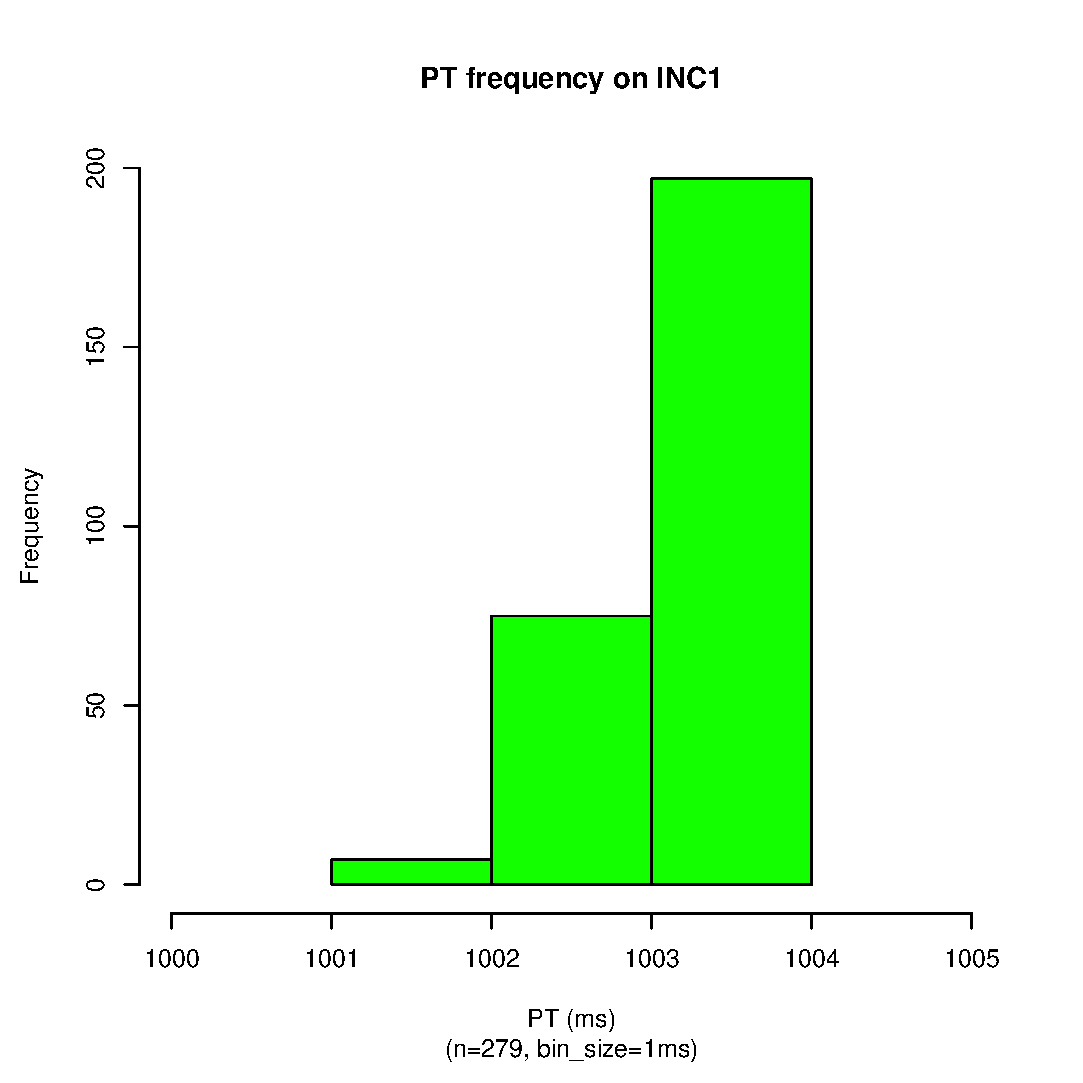
\includegraphics[scale=0.43]{sodb9/1_sec_pt_hist_v5.eps}
		\label{fig:inc1_hist_v5}
	}
	\subfigure[PT frequency on INC2]{
		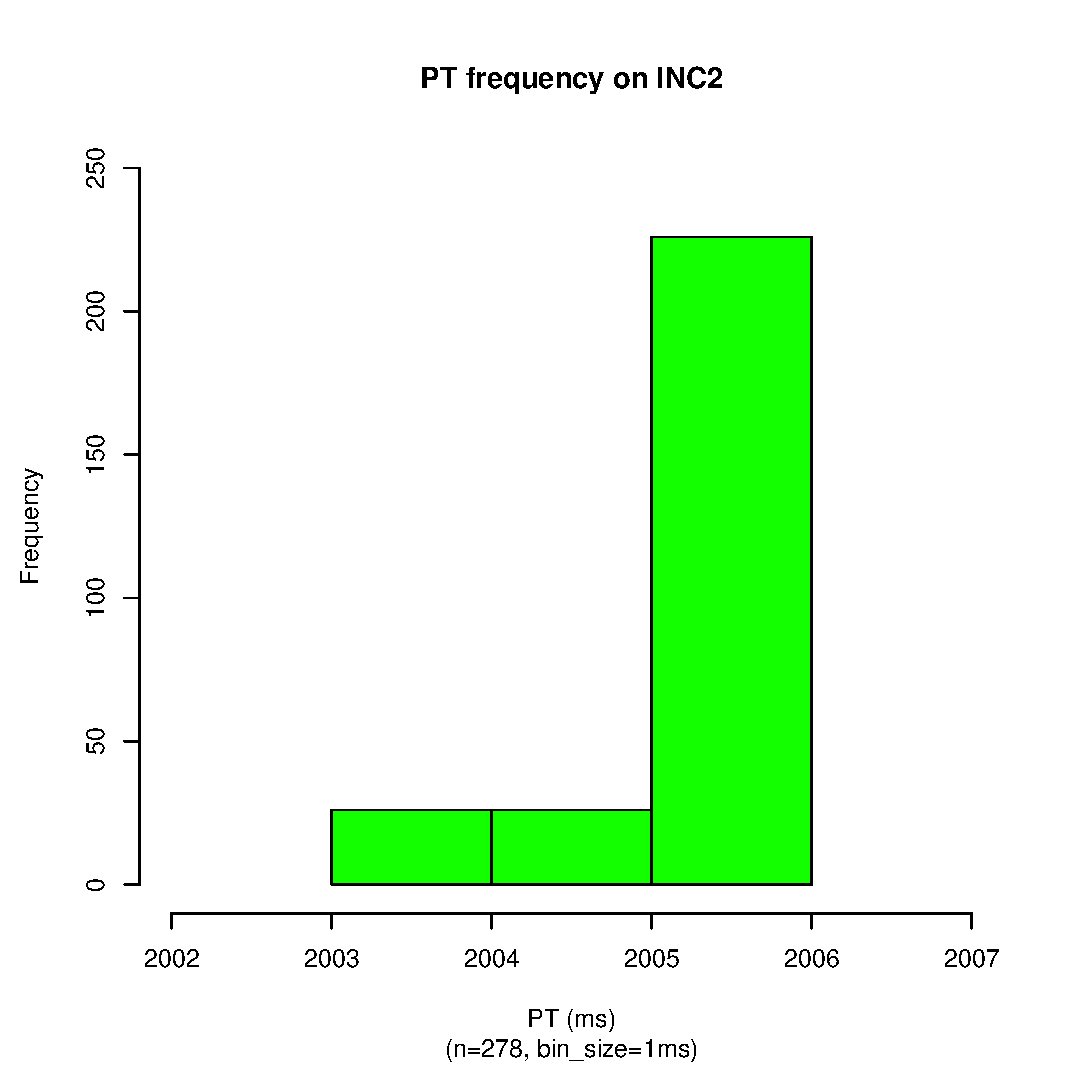
\includegraphics[scale=0.43]{sodb9/2_sec_pt_hist_v5.eps}
		\label{fig:inc2_hist_v5}
	}
	\subfigure[PT frequency on INC4]{
		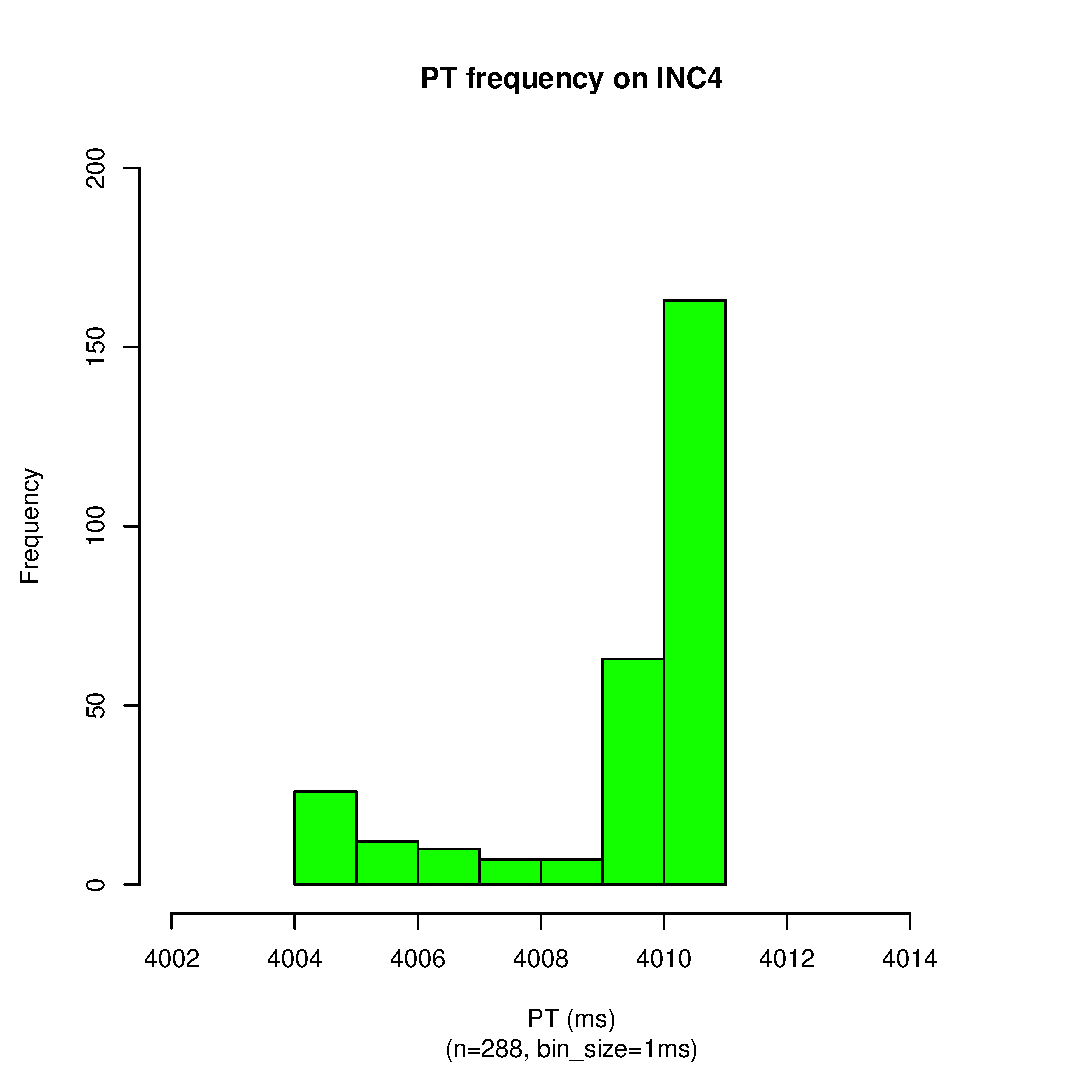
\includegraphics[scale=0.43]{sodb9/4_sec_pt_hist_v5.eps}
		\label{fig:inc4_hist_v5}
	}
	\subfigure[PT frequency on INC8]{
		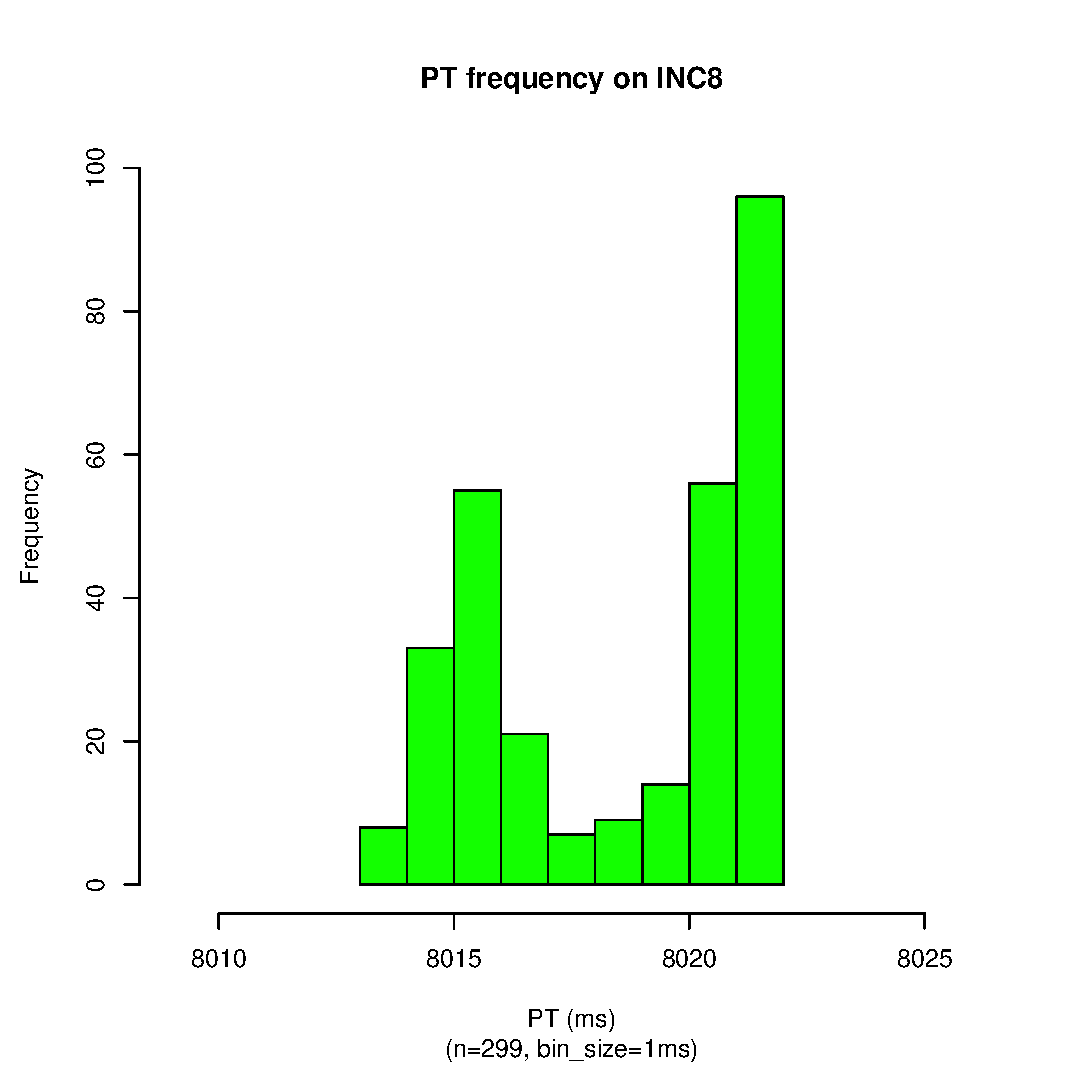
\includegraphics[scale=0.43]{sodb9/8_sec_pt_hist_v5.eps}
		\label{fig:inc8_hist_v5}
	}
	\caption{PT Histograms of INC1 ... INC8~\label{fig:s9_pt_hist1}}
\end{figure}

\begin{figure}[hp!]
	\centering
	\subfigure[PT frequency on INC16]{
		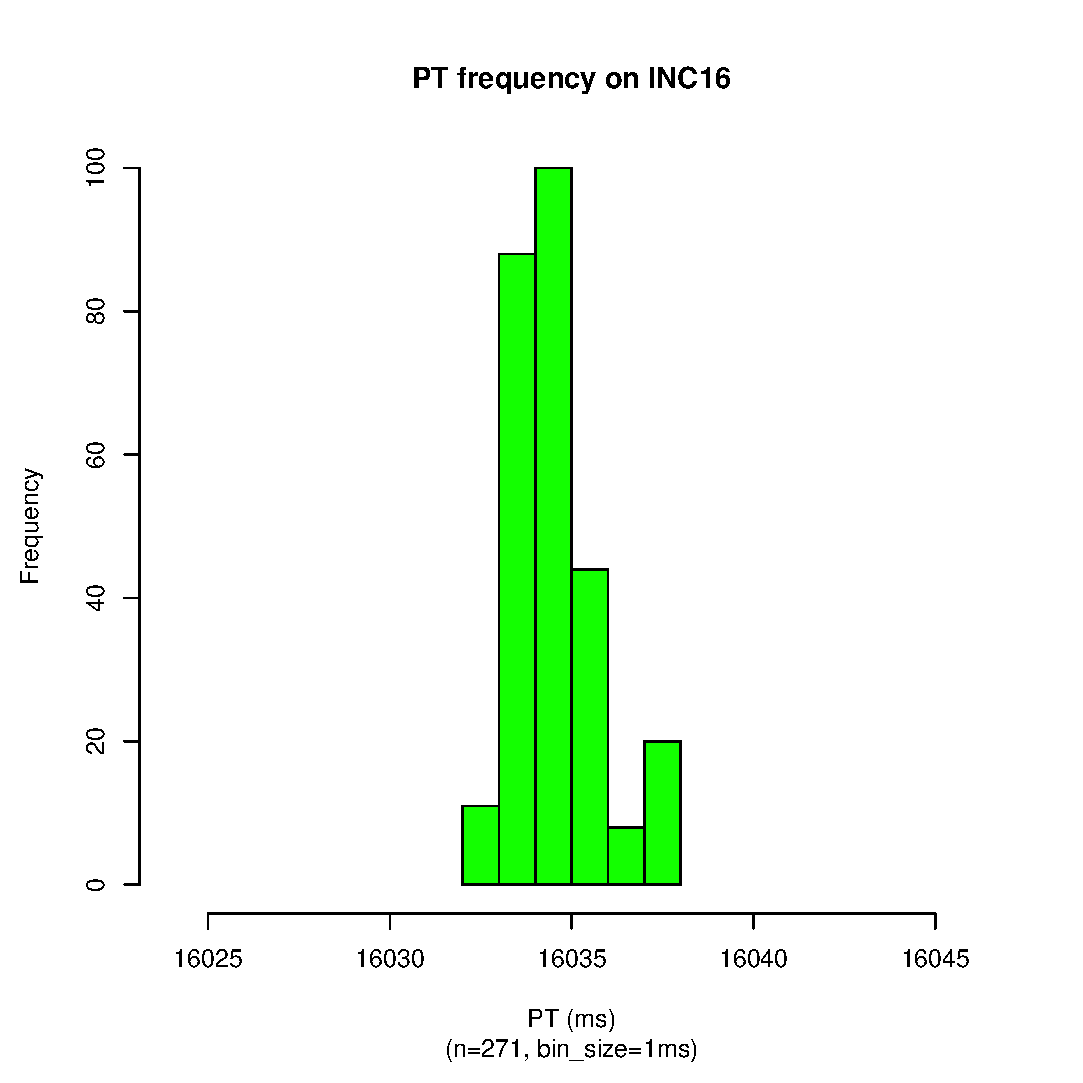
\includegraphics[scale=0.43]{sodb9/16_sec_pt_hist_v5.eps}
		\label{fig:inc16_hist_v5}
	}
	\subfigure[PT frequency on INC32]{
		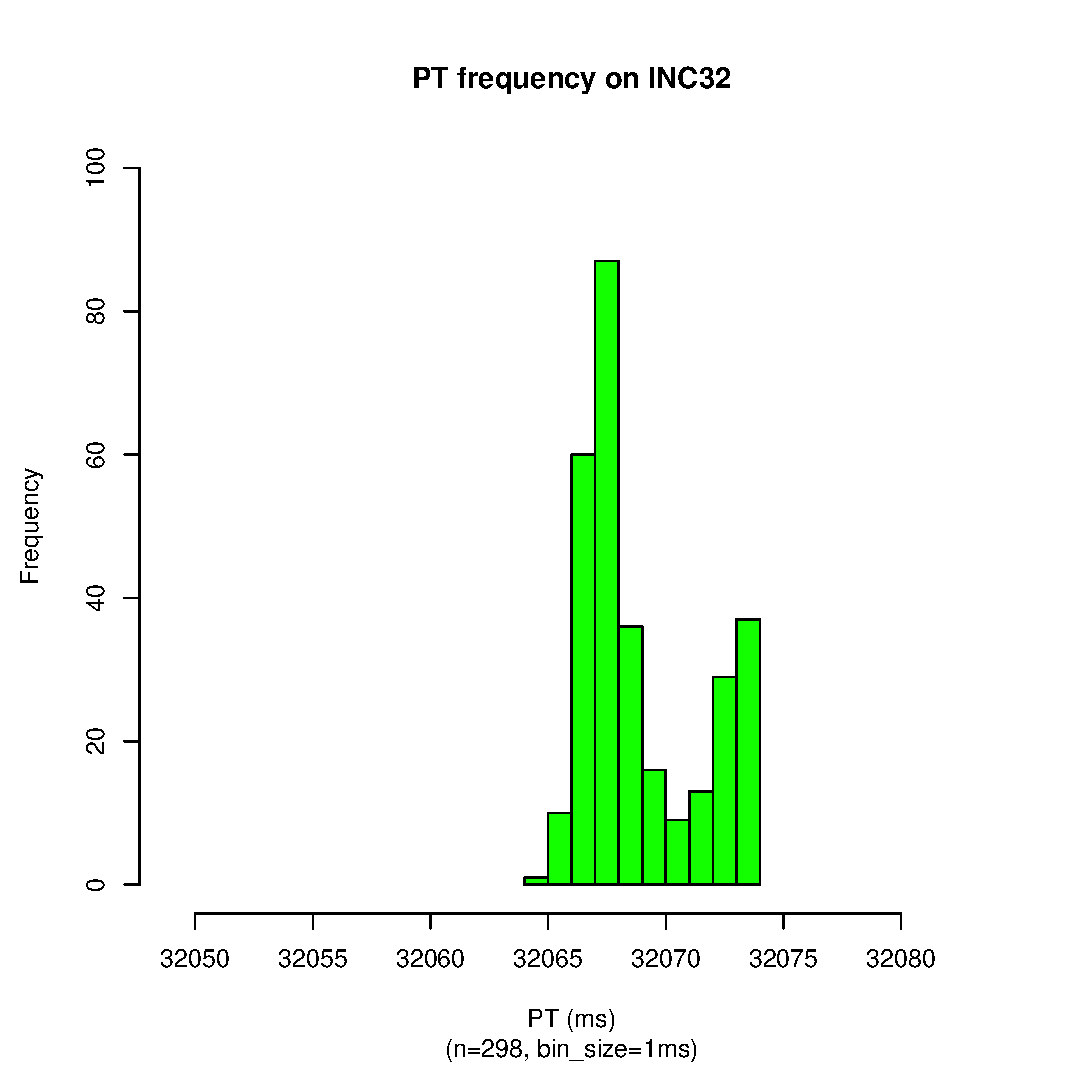
\includegraphics[scale=0.43]{sodb9/32_sec_pt_hist_v5.eps}
		\label{fig:inc32_hist_v5}
	}
	\subfigure[PT frequency on INC64]{
		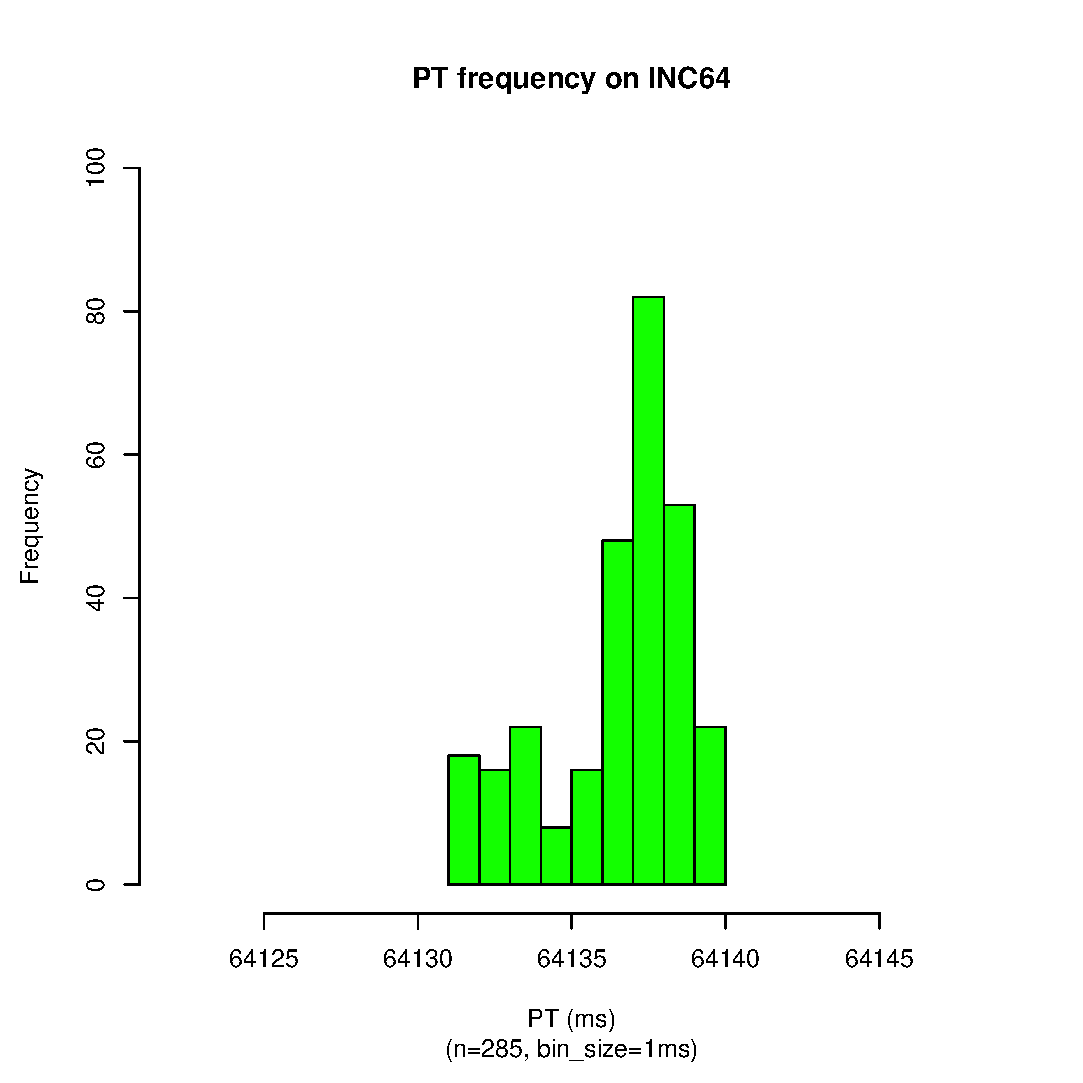
\includegraphics[scale=0.43]{sodb9/64_sec_pt_hist_v5.eps}
		\label{fig:inc64_hist_v5}
	}
	\caption{PT Histograms of INC16 ... INC64\label{fig:s9_pt_hist2}}
\end{figure}

\begin{figure}[hp!]
	\centering
	\subfigure[PT frequency on INC128]{
		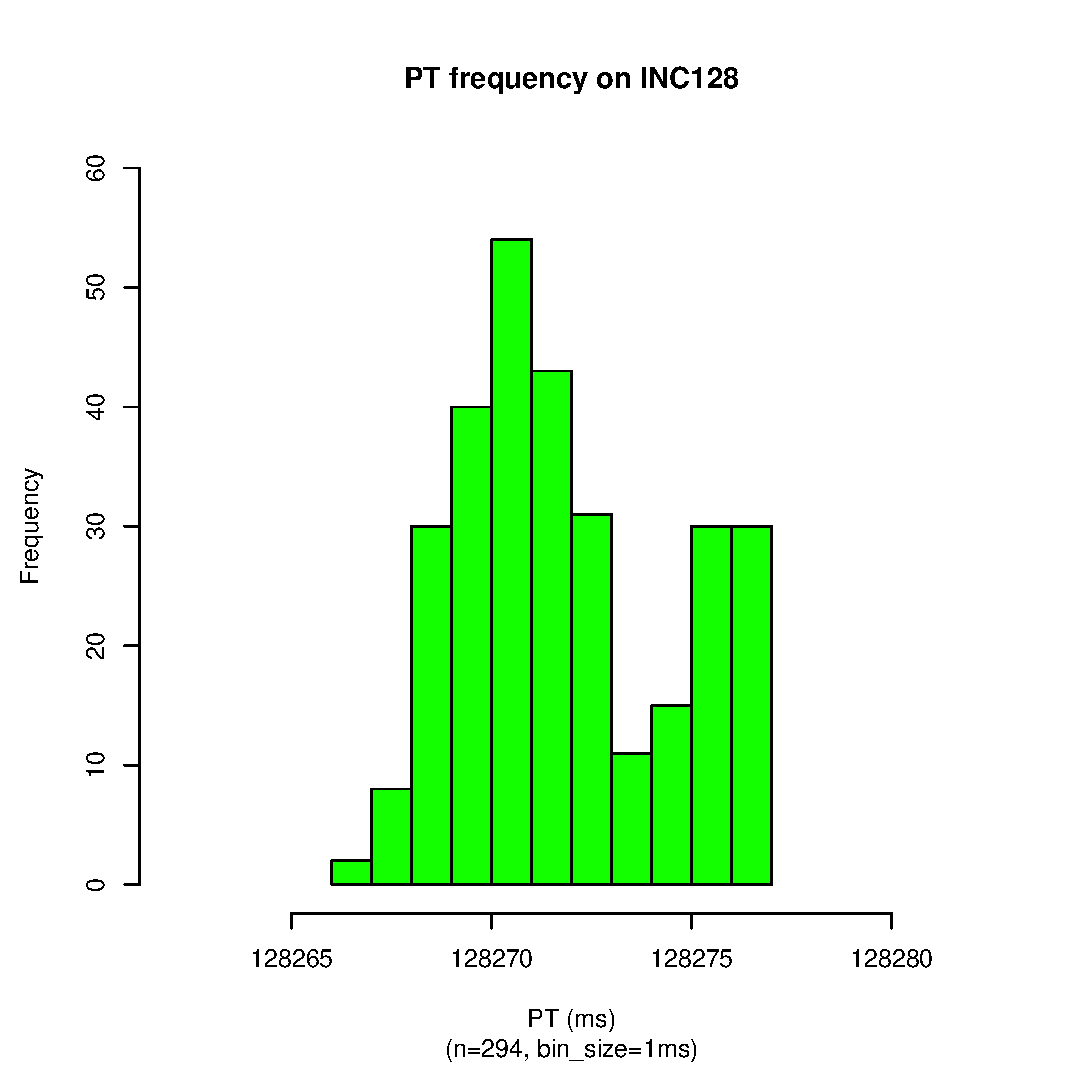
\includegraphics[scale=0.43]{sodb9/128_sec_pt_hist_v5.eps}
		\label{fig:inc128_hist_v5}
	}
	\subfigure[PT frequency on INC256]{
		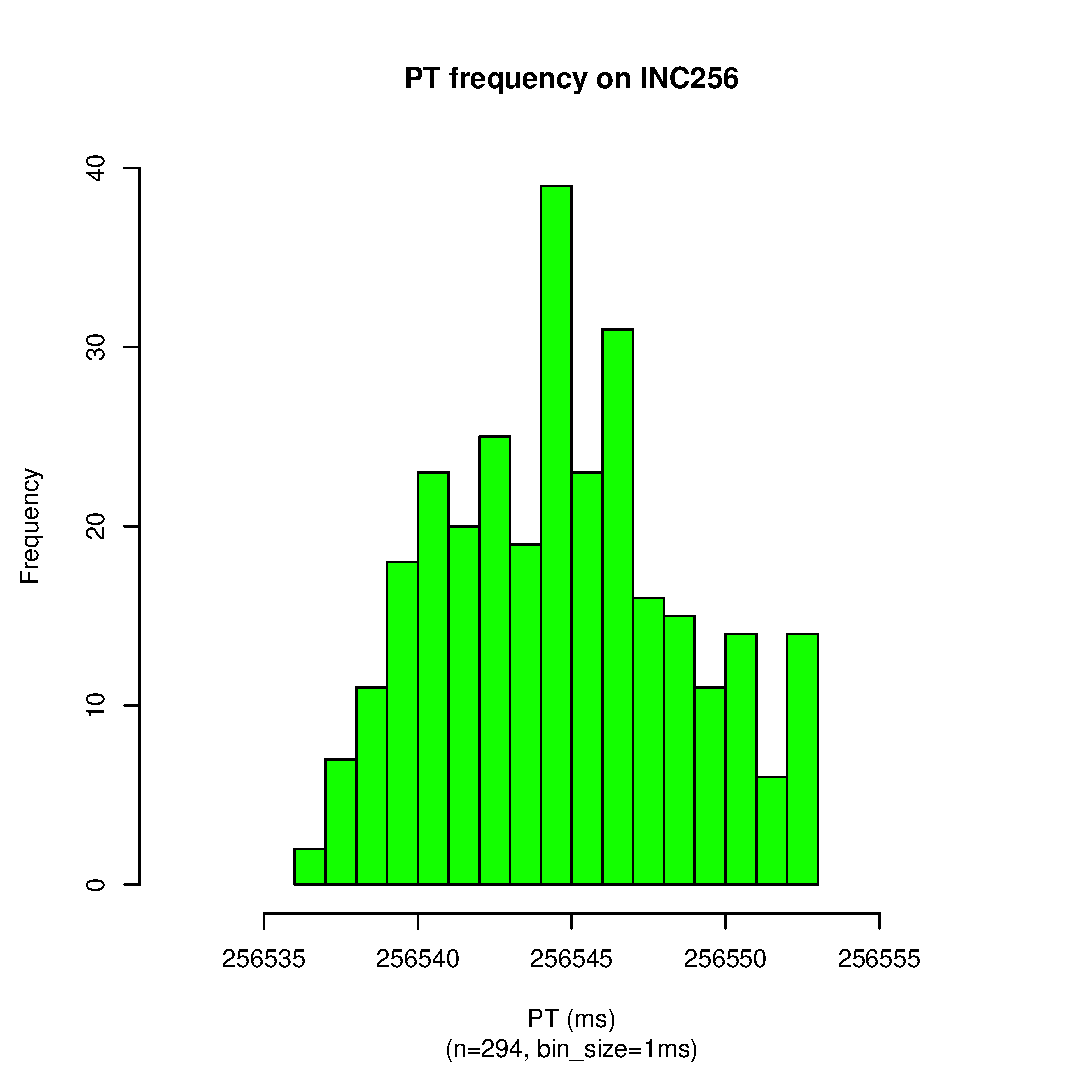
\includegraphics[scale=0.43]{sodb9/256_sec_pt_hist_v5.eps}
		\label{fig:inc256_hist_v5}
	}
	\subfigure[PT frequency on INC512]{
		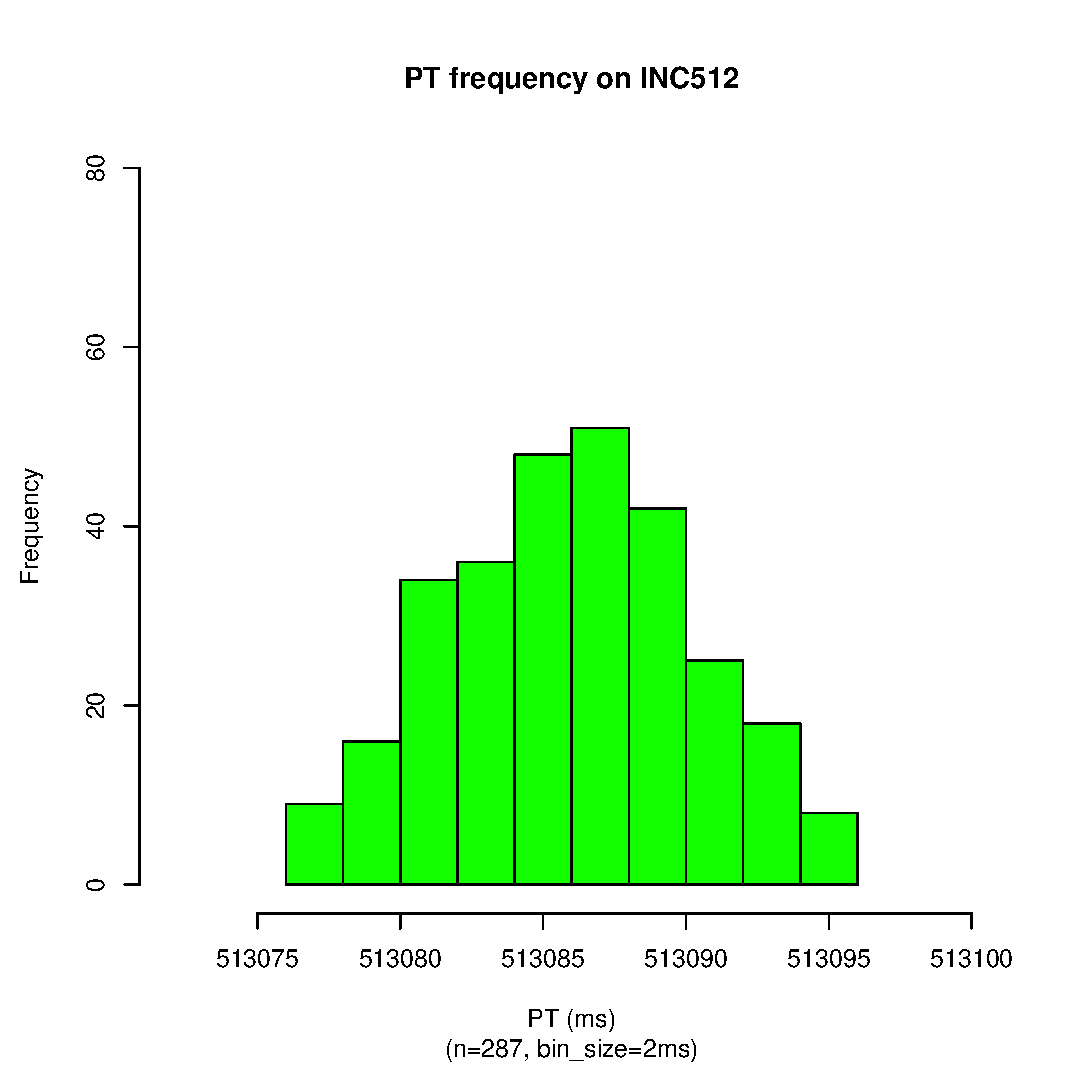
\includegraphics[scale=0.43]{sodb9/512_sec_pt_hist_v5.eps}
		\label{fig:inc512_hist_v5}
	}
	\subfigure[PT frequency on INC1024]{
		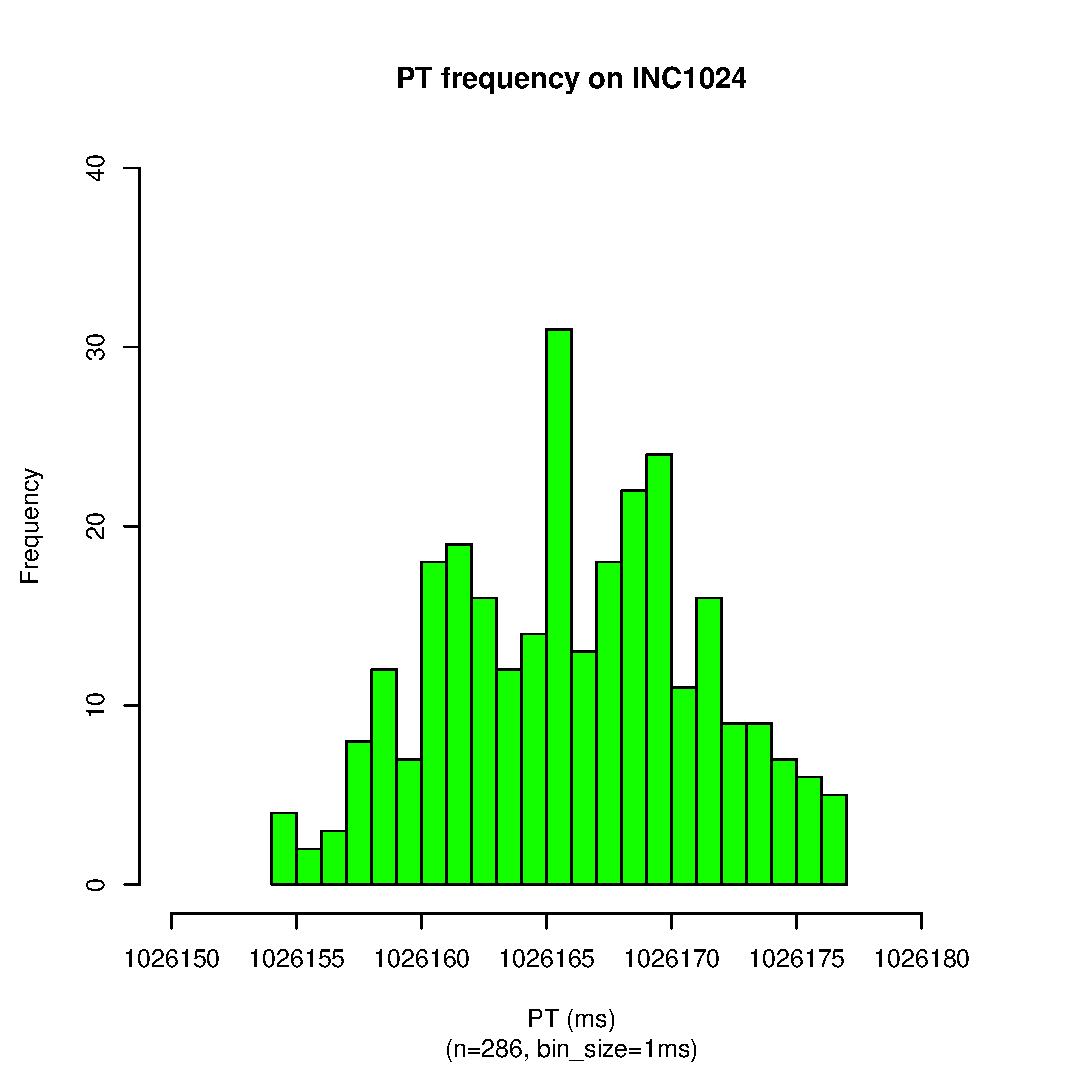
\includegraphics[scale=0.43]{sodb9/1024_sec_pt_hist_v5.eps}
		\label{fig:inc1024_hist_v5}
	}
	\caption{PT Histograms of INC256 ... INC1024~\label{fig:s9_pt_hist3}}
\end{figure}

\begin{figure}[hp!]
	\centering
	\subfigure[PT frequency on INC2048]{
		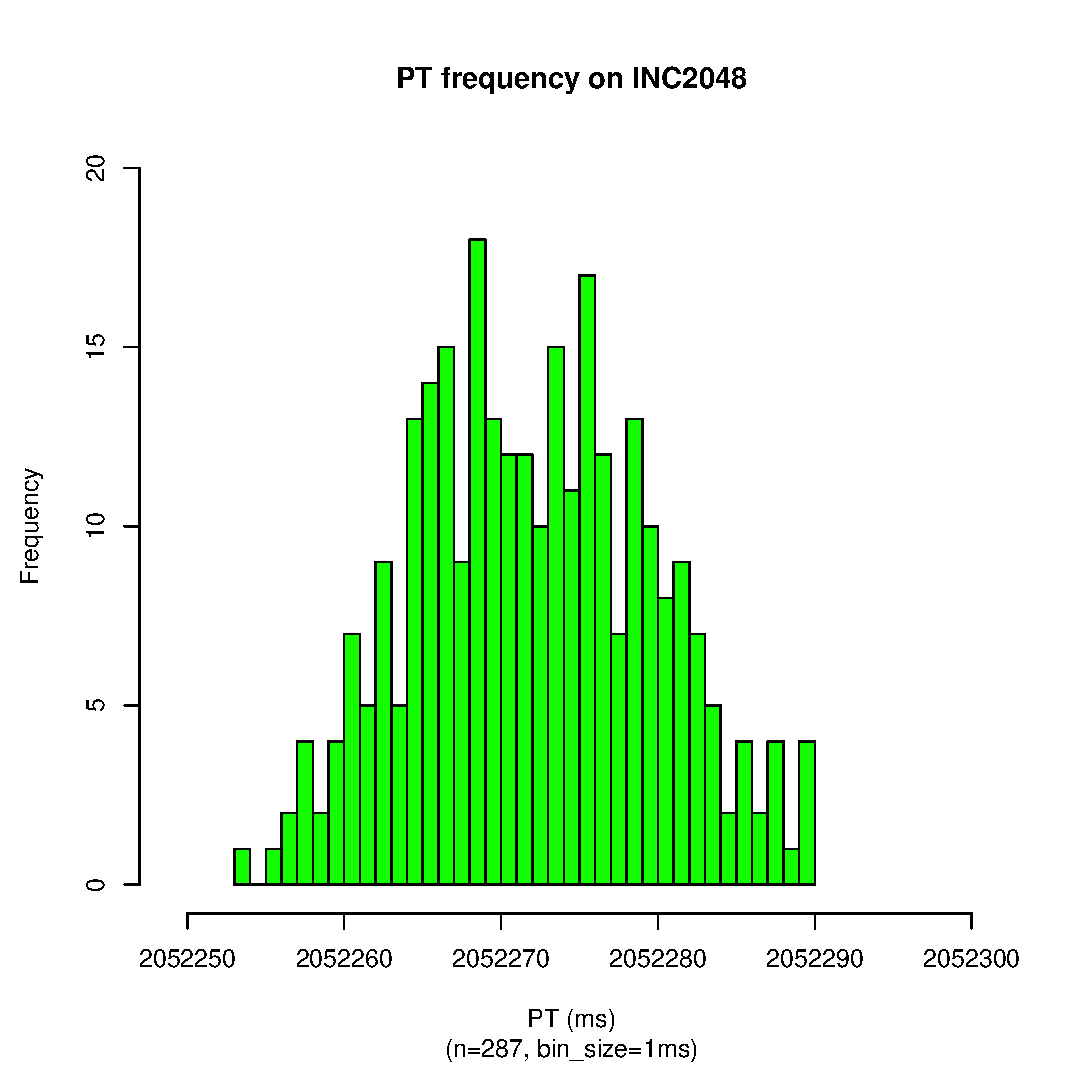
\includegraphics[scale=0.43]{sodb10/2048_sec_pt_hist_v5.eps}
		\label{fig:inc2048_hist_v5}
	}
	\subfigure[PT frequency on INC4096]{
		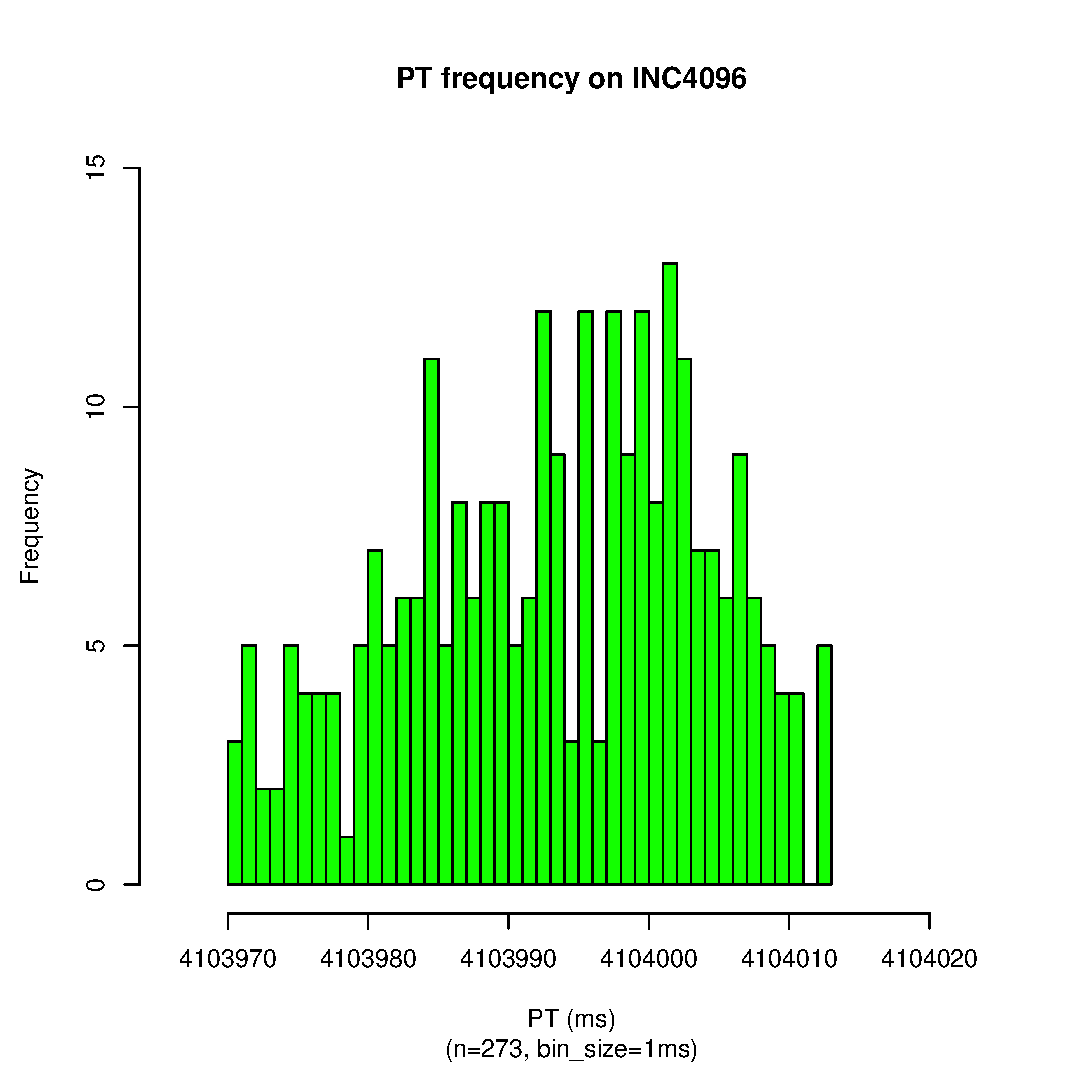
\includegraphics[scale=0.43]{sodb12/4096_sec_pt_hist_v5.eps}
		\label{fig:inc4096_hist_v5}
	}
	\subfigure[PT frequency on INC8192]{
		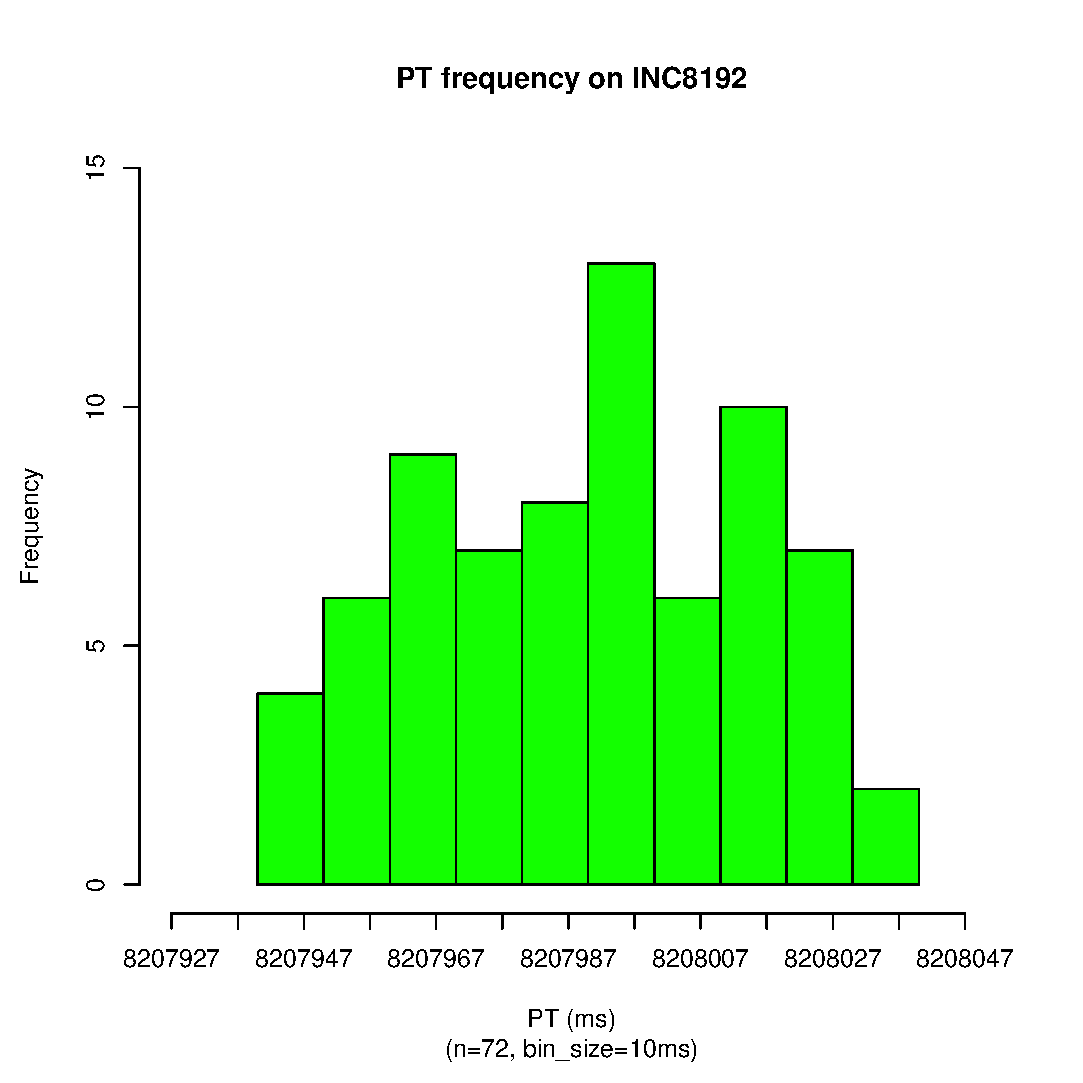
\includegraphics[scale=0.43]{sodb12/8192_sec_pt_hist2_v5.eps}
		\label{fig:inc8192_hist_v5}
	}
	\subfigure[PT frequency on INC16384]{
		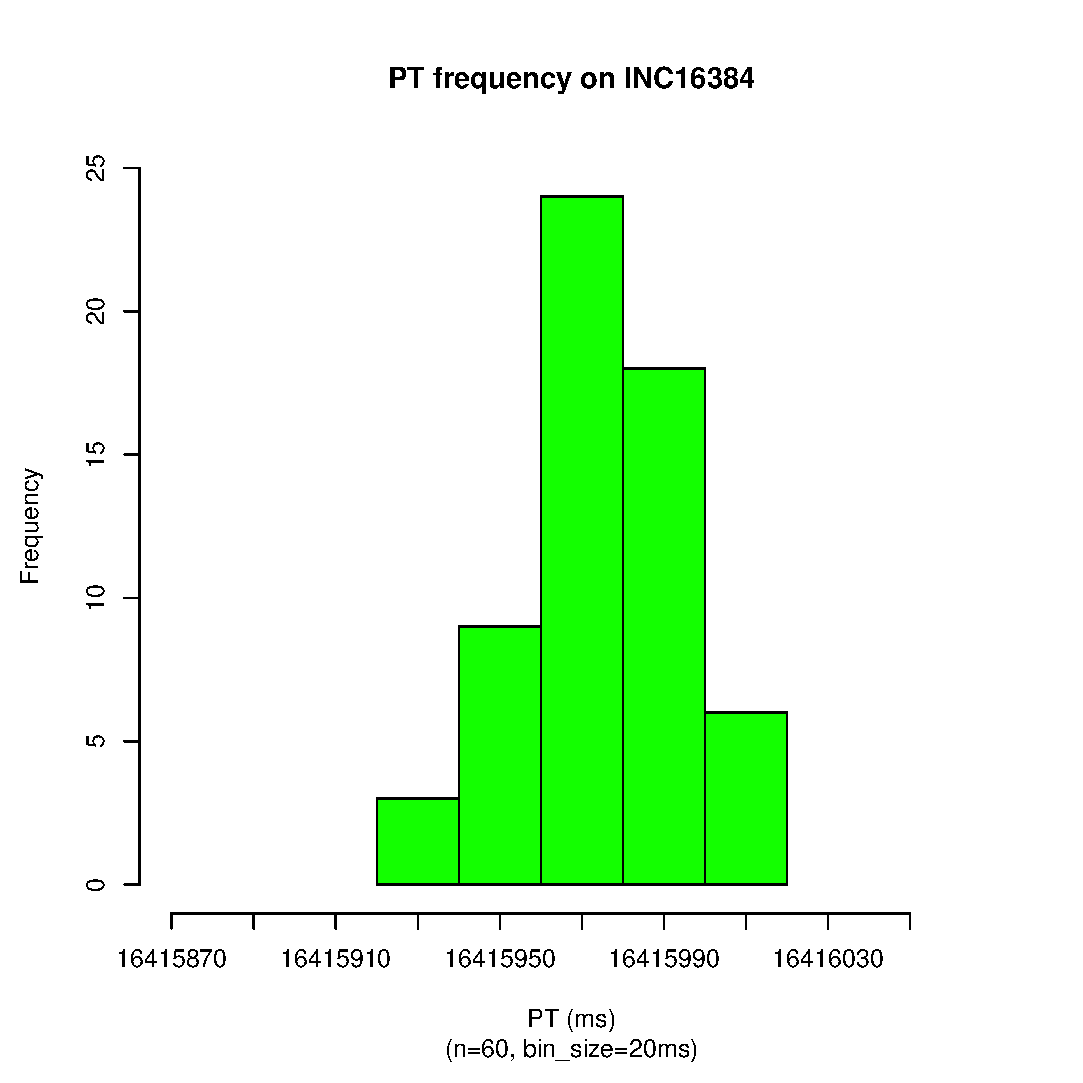
\includegraphics[scale=0.43]{sodb12/16384_sec_pt_hist2_v5.eps}
		\label{fig:inc16384_hist_v5}
	}
	\caption{PT Histograms of INC2048 and INC16384~\label{fig:s9_pt_hist4}}
\end{figure}

%\pagebreak
%
%\begin{figure}[hp!]
%	\centering
%	\subfigure[PT frequency on INC8192]{
%		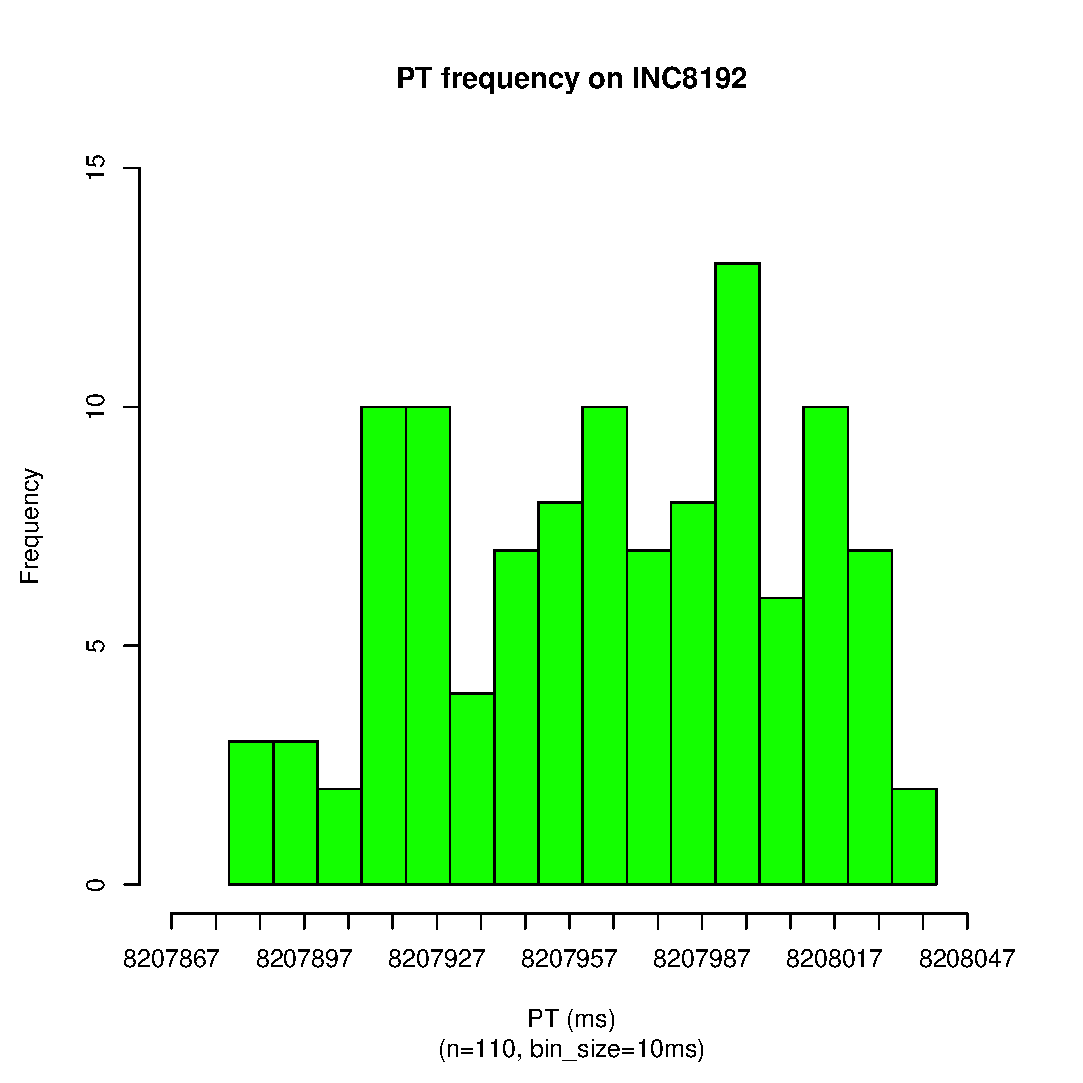
\includegraphics[scale=0.43]{sodb12/8192_sec_pt_hist_v5.eps}
%		\label{fig:inc8192_hist_all_v5}
%	}
%	\subfigure[PT frequency on INC16384]{
%		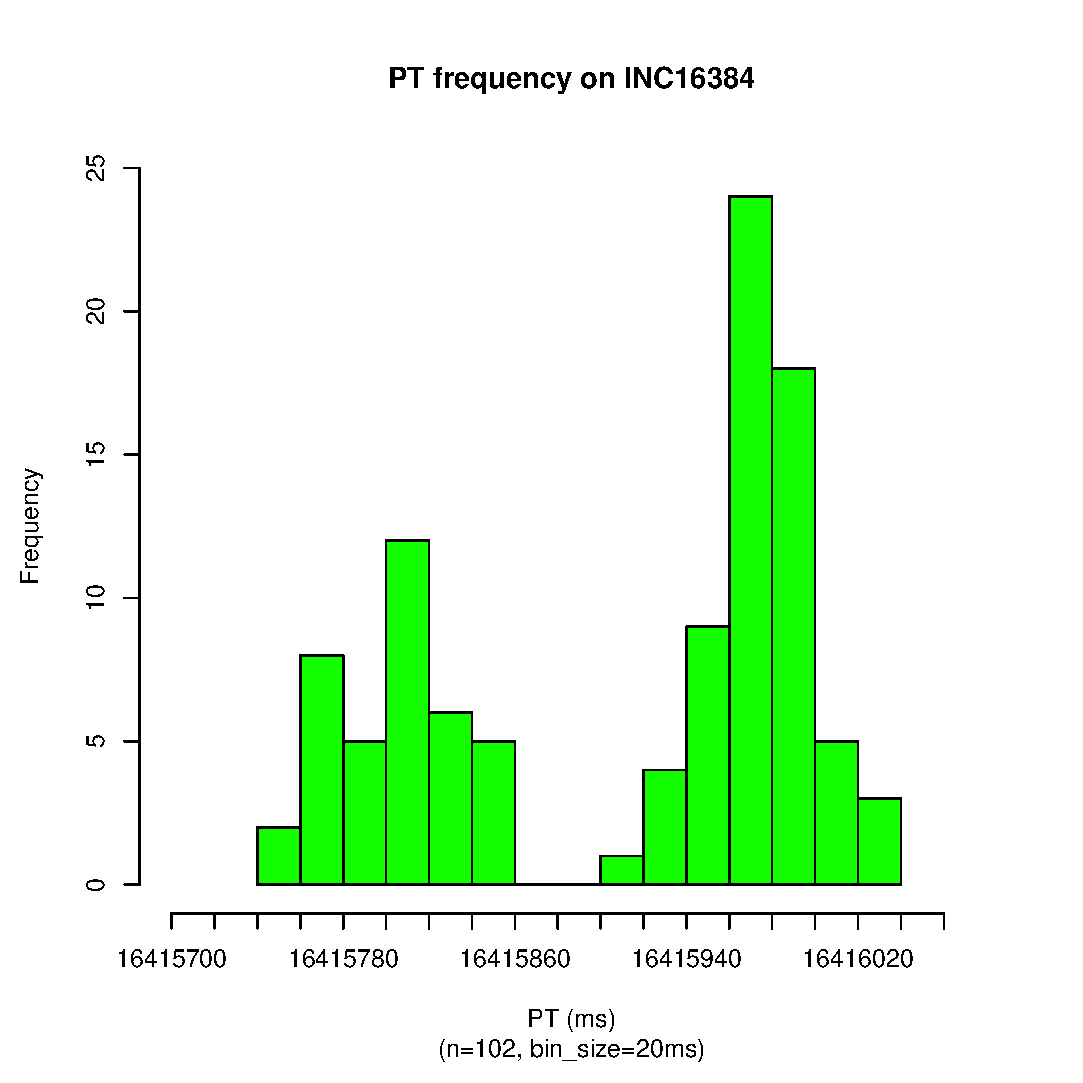
\includegraphics[scale=0.43]{sodb12/16384_sec_pt_hist_v5.eps}
%		\label{fig:inc16384_hist_all_v5}
%	}
%	\caption{PT Histograms of INC8192 and INC16384 [combined with 2015's run]~\label{fig:s9_pt_hist5}}
%\end{figure}

\pagebreak
\section{Analysis~\label{sec:hist_analysis}} 
In this section we gather all daemons observed and their statistics like minimum PT, maximum PT, average PT, and standard deviation of PT for each bin in Figures~\ref{fig:inc8_et_hist_v5} and~\ref{fig:inc16_et_hist_v5}.

\subsection{INC8}

\begin{table}[h]
\begin{center}
{\scriptsize
\begin{tabular}{l|l|l|l|l|l|l|l} \hline
TASK\_LEN  & BIN (ET) &  DAEMON   & MIN\_PT  &  MAX\_PT  &  AVG\_PT  &   STD\_PT & Counts \\ \hline
INC8     & 8014     & jbd2/md0-8     & 1     & 1     & 1     & 0     & 1\\ \hline
INC8     & 8014     & kslowd000     & 1     & 1     & 1     & 0     & 1\\ \hline
INC8     & 8014     & md0\_raid1     & 1     & 1     & 1     & 0     & 5\\ \hline
INC8     & 8014     & proc\_monitor     & 195     & 200     & 197.05     & 1.43     & 19\\ \hline \hline

INC8     & 8015     & jbd2/md0-8     & 1     & 1     & 1     & 0     & 1\\ \hline
INC8     & 8015     & kslowd001     & 1     & 1     & 1     & 0     & 1\\ \hline
INC8     & 8015     & md0\_raid1     & 1     & 1     & 1     & 0     & 1\\ \hline
INC8     & 8015     & proc\_monitor     & 198     & 198     & 198     & 0     & 4\\ \hline \hline

INC8     & 8016     & jbd2/md0-8     & 1     & 1     & 1     & 0     & 1\\ \hline
INC8     & 8016     & kblockd/0     & 1     & 1     & 1     & 0     & 1\\ \hline
INC8     & 8016     & kslowd000     & 1     & 1     & 1     & 0     & 31\\ \hline
INC8     & 8016     & kslowd001     & 1     & 1     & 1     & 0     & 36\\ \hline
INC8     & 8016     & md0\_raid1     & 1     & 1     & 1     & 0     & 19\\ \hline
INC8     & 8016     & proc\_monitor     & 196     & 198     & 196.72     & .93     & 68\\ \hline \hline

INC8     & 8017     & kslowd000     & 1     & 1     & 1     & 0     & 13\\ \hline
INC8     & 8017     & kslowd001     & 1     & 1     & 1     & 0     & 8\\ \hline
INC8     & 8017     & md0\_raid1     & 1     & 1     & 1     & 0     & 6\\ \hline
INC8     & 8017     & proc\_monitor     & 196     & 198     & 197.55     & .86     & 22\\ \hline \hline

INC8     & 8018     & kslowd000     & 1     & 1     & 1     & 0     & 4\\ \hline
INC8     & 8018     & kslowd001     & 1     & 1     & 1     & 0     & 6\\ \hline
INC8     & 8018     & md0\_raid1     & 1     & 1     & 1     & 0     & 5\\ \hline
INC8     & 8018     & proc\_monitor     & 196     & 198     & 197.4     & .97     & 10\\ \hline \hline

INC8     & 8019     & kslowd000     & 1     & 1     & 1     & 0     & 1\\ \hline
INC8     & 8019     & kslowd001     & 1     & 1     & 1     & 0     & 5\\ \hline
INC8     & 8019     & md0\_raid1     & 1     & 1     & 1     & 0     & 3\\ \hline
INC8     & 8019     & proc\_monitor     & 196     & 198     & 197     & 1.07     & 8\\ \hline \hline

INC8     & 8020     & jbd2/md0-8     & 1     & 1     & 1     & 0     & 1\\ \hline
INC8     & 8020     & kslowd000     & 1     & 1     & 1     & 0     & 3\\ \hline
INC8     & 8020     & kslowd001     & 1     & 1     & 1     & 0     & 1\\ \hline
INC8     & 8020     & md0\_raid1     & 1     & 1     & 1     & 0     & 8\\ \hline
INC8     & 8020     & proc\_monitor     & 196     & 198     & 196.73     & .98     & 33\\ \hline \hline

INC8     & 8021     & kslowd000     & 1     & 1     & 1     & 0     & 6\\ \hline
INC8     & 8021     & kslowd001     & 1     & 1     & 1     & 0     & 4\\ \hline
INC8     & 8021     & md0\_raid1     & 1     & 1     & 1     & 0     & 4\\ \hline
INC8     & 8021     & proc\_monitor     & 196     & 200     & 197.71     & 1.07     & 14\\ \hline \hline

INC8     & 8022     & cifsd     & 1     & 1     & 1     & 0     & 1\\ \hline
INC8     & 8022     & java     & 3     & 14     & 8.5     & 7.78     & 2\\ \hline
INC8     & 8022     & jbd2/md0-8     & 1     & 1     & 1     & 0     & 1\\ \hline
INC8     & 8022     & kslowd000     & 1     & 1     & 1     & 0     & 54\\ \hline
INC8     & 8022     & kslowd001     & 1     & 1     & 1     & 0     & 52\\ \hline
INC8     & 8022     & md0\_raid1     & 1     & 1     & 1     & 0     & 23\\ \hline
INC8     & 8022     & proc\_monitor     & 194     & 198     & 196.94     & 1     & 106\\ \hline \hline

INC8     & 8023     & kslowd000     & 1     & 1     & 1     & 0     & 6\\ \hline
INC8     & 8023     & kslowd001     & 1     & 1     & 1     & 0     & 9\\ \hline
INC8     & 8023     & md0\_raid1     & 1     & 1     & 1     & 0     & 10\\ \hline
INC8     & 8023     & proc\_monitor     & 196     & 198     & 197.87     & .52     & 15\\ \hline \hline

INC8     & 8046     & bash     & 7     & 7     & 7     & 0     & 1\\ \hline
INC8     & 8046     & jbd2/md0-8     & 1     & 1     & 1     & 0     & 1\\ \hline
INC8     & 8046     & kslowd000     & 1     & 1     & 1     & 0     & 1\\ \hline
INC8     & 8046     & proc\_monitor     & 198     & 198     & 198     & 0     & 1\\ \hline
INC8     & 8046     & sshd     & 1     & 14     & 5.33     & 7.51     & 3\\ \hline \hline
\end{tabular}
}
\end{center}
\caption{Daemons observed from the INC8 run~\label{tab:inc8_daemons}}
\end{table}

\pagebreak

\subsection{INC16}

\begin{table}[h]
\begin{center}
{\scriptsize
\begin{tabular}{l|l|l|l|l|l|l|l} \hline
TASK\_LEN  & BIN (ET) &  DAEMON   & MIN\_PT  &  MAX\_PT  &  AVG\_PT  &   STD\_PT & Counts \\ \hline
INC16     & 16034     & jbd2/md0-8     & 1     & 1     & 1     & 0     & 1\\ \hline
INC16     & 16034     & kslowd000     & 1     & 1     & 1     & 0     & 30\\ \hline
INC16     & 16034     & kslowd001     & 1     & 1     & 1     & 0     & 28\\ \hline
INC16     & 16034     & md0\_raid1     & 1     & 1     & 1     & 0     & 13\\ \hline
INC16     & 16034     & proc\_monitor     & 196     & 198     & 196.58     & .89     & 57\\ \hline \hline

INC16     & 16035     & java     & 2     & 3     & 2.75     & .5     & 4\\ \hline
INC16     & 16035     & kslowd000     & 1     & 1     & 1     & 0     & 15\\ \hline
INC16     & 16035     & kslowd001     & 1     & 1     & 1     & 0     & 19\\ \hline
INC16     & 16035     & md0\_raid1     & 1     & 1     & 1     & 0     & 7\\ \hline
INC16     & 16035     & proc\_monitor     & 196     & 200     & 197.47     & 1.13     & 34\\ \hline \hline

INC16     & 16036     & java     & 2     & 3     & 2.5     & .71     & 2\\ \hline
INC16     & 16036     & jbd2/md0-8     & 1     & 1     & 1     & 0     & 3\\ \hline
INC16     & 16036     & kslowd000     & 1     & 2     & 1.01     & .11     & 90\\ \hline
INC16     & 16036     & kslowd001     & 1     & 2     & 1.01     & .11     & 90\\ \hline
INC16     & 16036     & md0\_raid1     & 1     & 1     & 1     & 0     & 23\\ \hline
INC16     & 16036     & proc\_monitor     & 196     & 200     & 196.81     & 1.1     & 94\\ \hline \hline

INC16     & 16037     & cifsd     & 1     & 1     & 1     & 0     & 1\\ \hline
INC16     & 16037     & jbd2/md0-8     & 1     & 1     & 1     & 0     & 1\\ \hline
INC16     & 16037     & kslowd000     & 1     & 2     & 1.02     & .13     & 55\\ \hline
INC16     & 16037     & kslowd001     & 1     & 1     & 1     & 0     & 54\\ \hline
INC16     & 16037     & md0\_raid1     & 1     & 1     & 1     & 0     & 16\\ \hline
INC16     & 16037     & proc\_monitor     & 196     & 198     & 197.53     & .86     & 55\\ \hline \hline

INC16     & 16038     & cifsd     & 1     & 1     & 1     & 0     & 1\\ \hline
INC16     & 16038     & khugepaged     & 1     & 2     & 1.5     & .71     & 2\\ \hline
INC16     & 16038     & kslowd000     & 1     & 1     & 1     & 0     & 9\\ \hline
INC16     & 16038     & kslowd001     & 1     & 1     & 1     & 0     & 8\\ \hline
INC16     & 16038     & proc\_monitor     & 196     & 198     & 197.56     & .88     & 9\\ \hline \hline

INC16     & 16039     & kslowd000     & 1     & 1     & 1     & 0     & 9\\ \hline
INC16     & 16039     & kslowd001     & 1     & 1     & 1     & 0     & 10\\ \hline
INC16     & 16039     & md0\_raid1     & 1     & 1     & 1     & 0     & 7\\ \hline
INC16     & 16039     & proc\_monitor     & 196     & 200     & 197.31     & 1.38     & 13\\ \hline \hline

INC16     & 16040     & khugepaged     & 1     & 1     & 1     & 0     & 1\\ \hline
INC16     & 16040     & kslowd000     & 1     & 1     & 1     & 0     & 8\\ \hline
INC16     & 16040     & kslowd001     & 1     & 1     & 1     & 0     & 8\\ \hline
INC16     & 16040     & md0\_raid1     & 1     & 1     & 1     & 0     & 1\\ \hline
INC16     & 16040     & proc\_monitor     & 195     & 198     & 196.64     & 1.12     & 11\\ \hline \hline

INC16     & 16041     & kslowd000     & 1     & 1     & 1     & 0     & 5\\ \hline
INC16     & 16041     & kslowd001     & 1     & 1     & 1     & 0     & 3\\ \hline
INC16     & 16041     & md0\_raid1     & 1     & 1     & 1     & 0     & 1\\ \hline
INC16     & 16041     & proc\_monitor     & 198     & 198     & 198     & 0     & 6\\ \hline \hline

INC16     & 16042     & java     & 3     & 16     & 9.5     & 9.19     & 2\\ \hline
INC16     & 16042     & kblockd/0     & 1     & 1     & 1     & 0     & 1\\ \hline
INC16     & 16042     & kslowd000     & 1     & 1     & 1     & 0     & 17\\ \hline
INC16     & 16042     & kslowd001     & 1     & 1     & 1     & 0     & 17\\ \hline
INC16     & 16042     & md0\_raid1     & 1     & 1     & 1     & 0     & 5\\ \hline
INC16     & 16042     & proc\_monitor     & 196     & 200     & 197.06     & 1.39     & 17\\ \hline \hline

INC16     & 16043     & jbd2/md0-8     & 1     & 1     & 1     & 0     & 1\\ \hline
INC16     & 16043     & kslowd000     & 1     & 1     & 1     & 0     & 4\\ \hline
INC16     & 16043     & kslowd001     & 1     & 1     & 1     & 0     & 4\\ \hline
INC16     & 16043     & md0\_raid1     & 1     & 1     & 1     & 0     & 1\\ \hline
INC16     & 16043     & proc\_monitor     & 196     & 198     & 197.5     & 1     & 4\\ \hline \hline

\end{tabular}
}
\end{center}
\caption{Daemons observed from the INC16 run~\label{tab:inc16_daemons}}
\end{table}

\pagebreak
\section{Histograms with 10,000 Samples~\label{sec:10k_hist}}  
In this further evaluation we run INC8 and INC16 10,000 times. 
We render histograms based on the data from those two 10k runs. 

\subsection{INC8}

\begin{figure}[hp!]
	\centering
	\subfigure[ET frequency]{
		\includegraphics[scale=0.43]{sodb9_10k/8_sec_10k_et_hist_v5.eps}
		\label{fig:inc8_10k_et_hist_v5}
	}
	\subfigure[PT frequency]{
		\includegraphics[scale=0.43]{sodb9_10k/8_sec_10k_pt_hist_v5.eps}
		\label{fig:inc8_10k_pt_hist_v5}
	}
	\caption{Histograms of INC8 with 10,000 Samples~\label{fig:inc8_10k}}
\end{figure}

\subsection{INC16}

\begin{figure}[hp!]
	\centering
	\subfigure[ET frequency]{
		\includegraphics[scale=0.43]{sodb10_10k/16_sec_10k_et_hist_v5.eps}
		\label{fig:inc16_10k_et_hist_v5}
	}
	\subfigure[PT frequency]{
		\includegraphics[scale=0.43]{sodb10_10k/16_sec_10k_pt_hist_v5.eps}
		\label{fig:inc16_10k_pt_hist_v5}
	}
	\caption{Histograms of INC16 with 10,000 Samples~\label{fig:inc16_10k}}
\end{figure}

%In this section we gather all daemons observed and their statistics like minimum PT, maximum PT, average PT, and standard deviation of PT for each bin in Figures~\ref{fig:inc8_et_hist_v5} and~\ref{fig:inc16_et_hist_v5}.
